\documentclass[11pt]{article}
\usepackage[english]{babel}
\usepackage[utf8x]{inputenc}
\usepackage{amsmath}
\usepackage{graphicx}
\usepackage[colorinlistoftodos]{todonotes}
\usepackage{listings}
\usepackage[hmargin=2cm]{geometry}
\usepackage{color} 
\definecolor{codegreen}{rgb}{0,0.6,0}
\definecolor{codegray}{rgb}{0.5,0.5,0.5}
\definecolor{codepurple}{rgb}{0.58,0,0.82}
\definecolor{backcolour}{rgb}{0.95,0.95,0.92} 
\lstdefinestyle{mystyle}{
    backgroundcolor=\color{backcolour},   
    commentstyle=\color{codegreen},
    keywordstyle=\color{magenta},
    numberstyle=\tiny\color{codegray},
    stringstyle=\color{codepurple},
    basicstyle=\footnotesize,
    breakatwhitespace=false,         
    breaklines=true,                 
    captionpos=b,                    
    keepspaces=true,                 
    numbers=left,                    
    numbersep=5pt,                  
    showspaces=false,                
    showstringspaces=false,
    showtabs=false,                  
    tabsize=2
}
\lstset{style=mystyle}
\begin{document}
\begin{titlepage}
\newcommand{\HRule}{\rule{\linewidth}{0.5mm}}
\center
\textsc{\LARGE Universidad de Granada}\\[1.5cm] % Name of your university/college
\textsc{\Large Algorítmica}\\[0.5cm] % Major heading such as course name
\textsc{\large Memoria de Prácticas}\\[0.5cm] % Minor heading such as course title
\HRule \\[0.4cm]
{ \huge \bfseries Práctica I: Eficiencia}\\[0.4cm] % Title of your document
\HRule \\[1.5cm]
\begin{minipage}{0.4\textwidth}
\begin{flushleft} \large
\emph{Autores:}\\
Elena Merelo Molina \\ Antonio Gámiz Delgado\textsc{} % Your name
\end{flushleft}
\end{minipage}
~
\begin{minipage}{0.4\textwidth}
\begin{flushright} \large
\emph{} \\
\textsc{} % Supervisor's Name
\end{flushright}
\end{minipage}\\[2cm]
{\large 17 de Marzo}\\[2cm] % Date, change the \today to a set date if you want to be precise

\includegraphics{logo.png}\\[1cm]
\vfill % Fill the rest of the page with whitespace
\end{titlepage}

\section{Análisis de la Eficiencia}


\subsection{Algoritmo de Inserción}
\begin{lstlisting}[language=C]
inline static void insercion(int T[], int num_elem)
{
  insercion_lims(T, 0, num_elem);
}

static void insercion_lims(int T[], int inicial, int final)
{
  int i, j;
  int aux;
  for (i = inicial + 1; i < final; i++) {
    j = i;
    while ((T[j] < T[j-1]) && (j > 0)) {
      aux = T[j];
      T[j] = T[j-1];
      T[j-1] = aux;
      j--;
    };
  };
}
\end{lstlisting}

Vamos a estudiar el peor caso que se le podría presentar al algoritmo de inserción, es decir, que el vector estuviera ordenado en orden inverso (de mayor a menor).

Como vemos en la línea 5, siempre se llama al método con los argumentos $0$ y $num\_elem$, por lo que a partir de ahora para nosotros, $inicial$ será $0$ y $final$ será $n$.

La mayor parte del tiempo de ejecución se emplea en el cuerpo del bucle $while$ interno. Ese trozo de código se puede acotar por una constante $a$. Por lo tanto, las líneas 15-19 se ejecutan un número de veces dependiente del bucle externo, exactamente $i$ veces (ya que estamos suponiendo que nos encontramos en el peor caso). El bucle externo se ejecuta exactamente $n$ veces, por lo que nos queda:

\[T(n)=\sum_{i=1}^{n-1}\sum_{j=1}^{i}a=a\sum_{i=0}^{n-1}\sum_{j=1}^{i}1=a\sum_{i=0}^{n-1}i=a\frac{n(n-1)}{2}\]
Por lo que vemos que $T(n)\in O(n^2)$ o cuadrático.

\subsection{Algoritmo QuickSort}
\begin{lstlisting}[language=C]

static void heapsort(int T[], int num_elem)
{
  int i;
  for (i = num_elem/2; i >= 0; i--)
    reajustar(T, num_elem, i);
  for (i = num_elem - 1; i >= 1; i--)
    {
      int aux = T[0];
      T[0] = T[i];
      T[i] = aux;
      reajustar(T, i, 0);
    }
} 

static void reajustar(int T[], int num_elem, int k)
{
  int j;
  int v;
  v = T[k];
  bool esAPO = false;
  while ((k < num_elem/2) && !esAPO)
    {
      j = k + k + 1;

      if ((j < (num_elem - 1)) && (T[j] < T[j+1])) j++;
      if (v >= T[j]) esAPO = true;
      
      T[k] = T[j];
      k = j;
    }
  T[k] = v;
}
\end{lstlisting}

Vemos que en el primer bucle de la función $heapsort$ aparece la función $reajustar$, por lo que vamos a calcular su eficiencia primero. 

Vemos que el cuerpo del bucle $while$ consume la mayor parte del tiempo de ejecución. El cuerpo de bucle se puede acotar por una constante $b$. Como vemos en la línea 22, el bucle empieza en $k$ y termina en $\frac{n}{2}$, pero $k$ no avanza de 1 en 1, sino de $2k+1$ en $2k+1$, por lo que como mucho se ejecutará $\log(n/2)$ veces. Por lo que $R(n) \in O(\log(n))$, siendo $K(n)$ la función de eficiencia de la función $reajustar$.
Una vez conocida la eficiencia de la función $reajustar$, pasamos a estudiar el primer bucle de la función $heapsort$. Va desde $n/2$ hasta $0$, así que se ejecuta $n/2$ veces, y en cada una de esas veces ejecuta la función $reajustar$, por lo que encontes su eficiencia es $\frac{nlog(n)}{2}$. El segundo bucle se ejecuta $n-1$ veces, por lo que nos queda:
\[T(n)=\frac{nlog(n)}{2}+(n-1)\]
Por lo que $T(n)\in O(n\log(n))$.

\subsection{Algoritmo de Floyd}
\begin{lstlisting}[language=C]
void Floyd(int **M, int dim)
{
	for (int k = 0; k < dim; k++)
	  for (int i = 0; i < dim;i++)
	    for (int j = 0; j < dim;j++)
	      {
				int sum = M[i][k] + M[k][j];    	
		    M[i][j] = (M[i][j] > sum) ? sum : M[i][j];
	      }
}
\end{lstlisting}

Vemos que el cuerpo del tercer bucle $while$ anidado consume la mayor parte del tiempo de ejecución, por lo que lo acotamos por una constante $a$. Fácilmente vemos que el resto de bucles va desde 0 hasta $dim$, que podemos denominar $n$ para mayor facilidad. Por lo que evidentemente tenemos que la eficiencia de este algoritmo es $an^3$, es decir, $T(n)\in O(n^3)$.

\section{Eficiencia empírica}

En esta práctica vamos a estudiar la eficiencia empírica de los siguientes algoritmos:

\begin{center}
\begin{tabular}{| c | c |}
\hline
Algoritmo & Orden de Eficiencia \\ \hline
Burbuja & O$(n^2$) \\ \hline
Inserción & O$(n^2$) \\ \hline 
Selección & O$(n^2$) \\ \hline 
Mergesort & O$(n\log(n)$) \\ \hline 
Quicksort & O$(n\log(n)$) \\ \hline 
Heapsort & O$(n\log(n)$) \\ \hline
Floyd & O$(n^3)$ \\ \hline 
Hanoi & O$(2^n)$ \\ \hline 
\hline
\end{tabular}
\end{center}

Para el estudio de la eficiencia empírica hemos escrito un script \footnotetext{Adjuntamos el código del script pero no lo explicamos ya que creemos que no es el objetivo de esta práctica.} en $Python 2.7$ para facilitar el trabajo de la gestión de los datos. Primeramente añadimos a cada programa unas líneas de código y de esta manera medir el tiempo que ha tardado en ejecutarse. Luego compilamos cada programa con 3 opciones de optimización distintas (sin optimizar, con -O1 y con -O2) con g++, y una vez obtenidos los ejecutables, ejecutamos cada grupo de programas 25 veces con diferentes valores de $n$ (tamaño) para cada algoritmo y guardamos los resultados en varios archivos (los datos obtenidos se pueden ver en las tablas de abajo). Una vez hecho todo esto, ajustamos aplicando el método de mínimos cuadrados los datos con su orden de eficiencia:

\begin{enumerate}
\item $O(n^2)$: ajustada por la función $f(x)=ax^2+bx+c$
\item $O(n\log(n)$: ajustada por la función $f(x)=a\log(bn)+c$
\item $O(n^3)$: ajustada por la función $f(x)=ax^3+bx^2+cx+d$
\item $O(2^n)$: ajustada por la función $f(x)=a2^{bn}+c$
\end{enumerate}


Los valores obtenidos para los coeficientes $(a,b,c,d)$ aparecen en la legenda de las gráficas según la opción de optimización usada.

Las última gráfica de cada página muestra como varía la eficiencia del algoritmo en función de la opción de optimización usada.

A continuación mostramos todos los datos obtenidos junto a las gráficas de los algoritmos expuestos arriba:


\newpage
\subsection{Algoritmo burbuja (Elena)}
\begin{center}
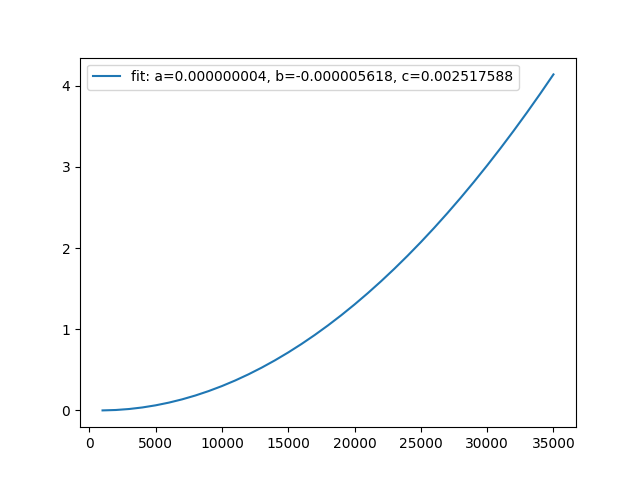
\includegraphics[width=.4\textwidth]{../graficos/burbuja/burbuja_elena.png}
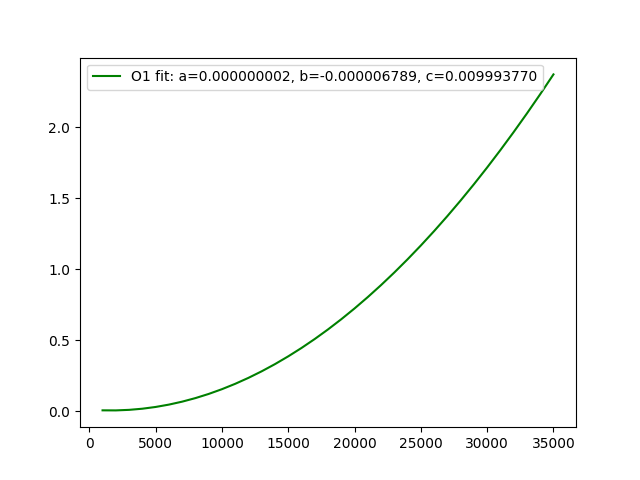
\includegraphics[width=.4\textwidth]{../graficos/burbuja/burbuja_O1_elena.png}
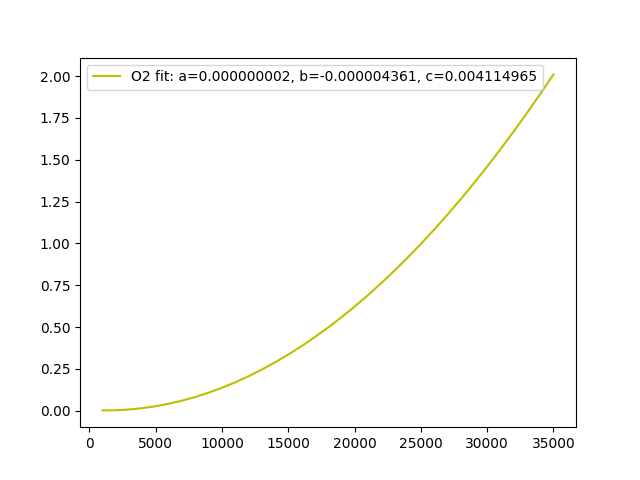
\includegraphics[width=.4\textwidth]{../graficos/burbuja/burbuja_O2_elena.png}
\end{center}
\begin{center}
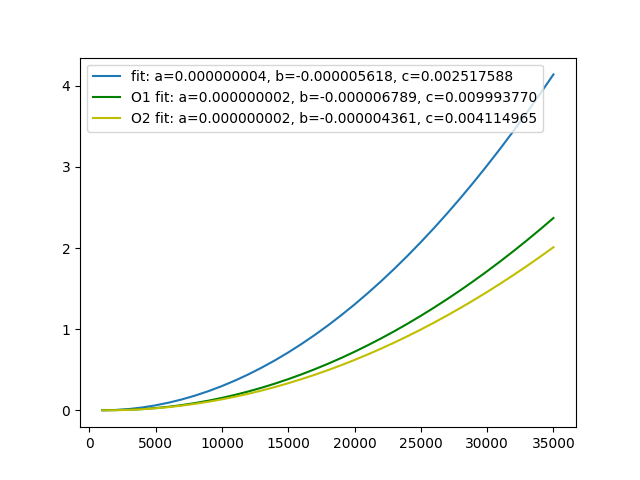
\includegraphics[width=.6\textwidth]{../graficos/burbuja/burbuja_juntas_elena.png}
\end{center}
\begin{center}
\begin{tabular}{| c | c | c | c |}
\hline
\textbf{N} & \textbf{O-} & \textbf{O1} & \textbf{O2} \\ \hline
1000 & 0.00224433 & 0.00102678 & 0.000791685 \\ \hline
2000 & 0.00855251 & 0.00366315 & 0.00327288 \\ \hline
3000 & 0.0197315 & 0.0089917 & 0.00777837 \\ \hline
4000 & 0.0372338 & 0.0179805 & 0.0159009 \\ \hline
5000 & 0.0612263 & 0.0307844 & 0.0272179 \\ \hline
6000 & 0.0931501 & 0.0467117 & 0.0426332 \\ \hline
7000 & 0.141121 & 0.0679487 & 0.0618318 \\ \hline
8000 & 0.189752 & 0.0933759 & 0.0797291 \\ \hline
9000 & 0.235398 & 0.122148 & 0.105121 \\ \hline
10000 & 0.293126 & 0.154214 & 0.136209 \\ \hline
11000 & 0.372834 & 0.193827 & 0.167798 \\ \hline
12000 & 0.434022 & 0.239529 & 0.202906 \\ \hline
13000 & 0.52755 & 0.278723 & 0.255706 \\ \hline
14000 & 0.608207 & 0.326521 & 0.286101 \\ \hline
15000 & 0.720389 & 0.387952 & 0.331906 \\ \hline
16000 & 0.805799 & 0.440765 & 0.388973 \\ \hline
17000 & 0.93492 & 0.508819 & 0.429878 \\ \hline
18000 & 1.03981 & 0.567453 & 0.503668 \\ \hline
19000 & 1.18039 & 0.642401 & 0.54615 \\ \hline
20000 & 1.3095 & 0.725319 & 0.62702 \\ \hline
21000 & 1.4486 & 0.800284 & 0.681884 \\ \hline
22000 & 1.57821 & 0.887376 & 0.75987 \\ \hline
23000 & 1.76802 & 0.970347 & 0.839553 \\ \hline
24000 & 1.89164 & 1.06591 & 0.913394 \\ \hline
25000 & 2.06779 & 1.17406 & 1.00485 \\ \hline
26000 & 2.25955 & 1.27417 & 1.08369 \\ \hline
27000 & 2.43821 & 1.36573 & 1.17166 \\ \hline
28000 & 2.61991 & 1.49046 & 1.27354 \\ \hline
29000 & 2.81486 & 1.59349 & 1.35703 \\ \hline
30000 & 3.01869 & 1.71685 & 1.45953 \\ \hline
31000 & 3.23556 & 1.84846 & 1.56174 \\ \hline
32000 & 3.45231 & 1.95537 & 1.68971 \\ \hline
33000 & 3.65181 & 2.0881 & 1.75914 \\ \hline
34000 & 3.91054 & 2.24322 & 1.8894 \\ \hline
35000 & 4.12783 & 2.3636 & 2.01188 \\ \hline
\hline
\end{tabular}
\end{center}

\newpage
\subsection{Algoritmo burbuja (Antonio)}
\begin{center}
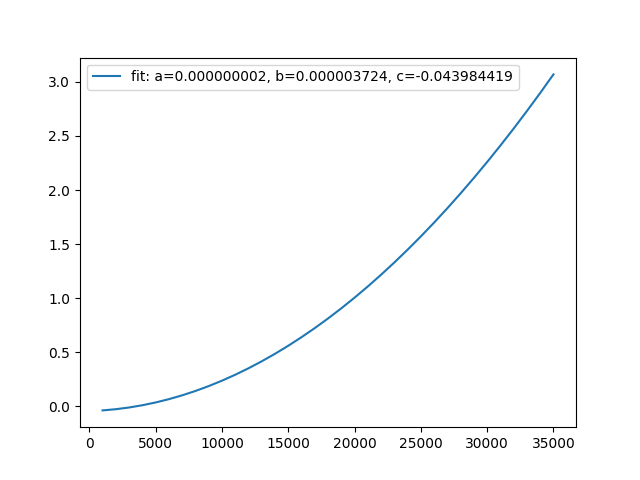
\includegraphics[width=.4\textwidth]{../graficos/burbuja/burbuja_antonio.png}
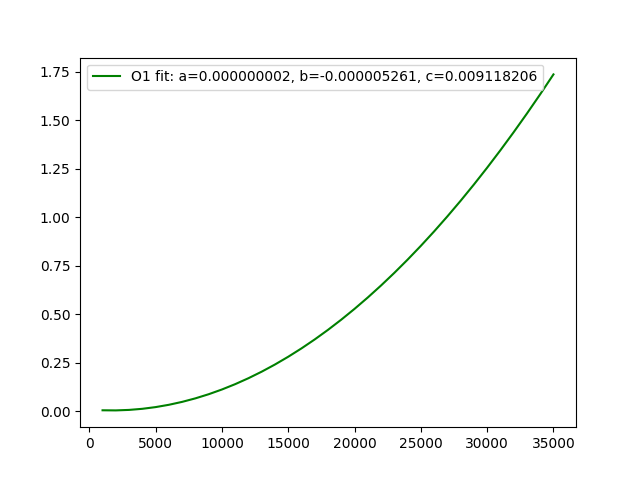
\includegraphics[width=.4\textwidth]{../graficos/burbuja/burbuja_O1_antonio.png}
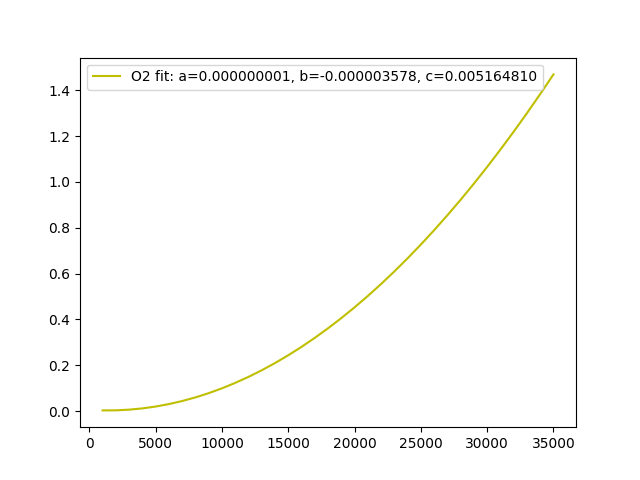
\includegraphics[width=.4\textwidth]{../graficos/burbuja/burbuja_O2_antonio.png}
\end{center}
\begin{center}
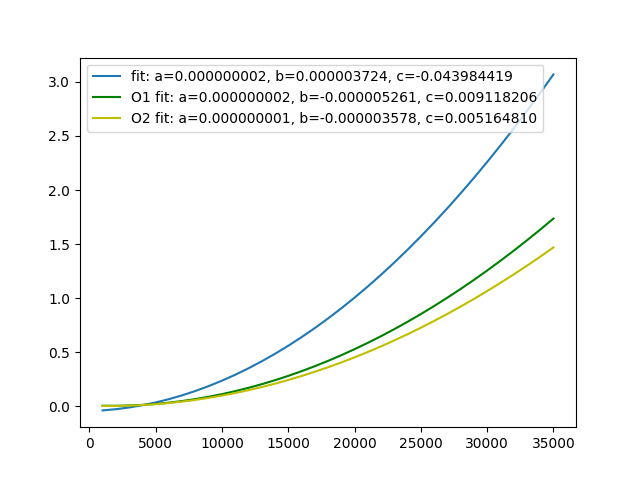
\includegraphics[width=.6\textwidth]{../graficos/burbuja/burbuja_juntas_antonio.png}
\end{center}
\begin{center}
\begin{tabular}{| c | c | c | c |}
\hline
\textbf{N} & \textbf{O-} & \textbf{O1} & \textbf{O2} \\ \hline
1000 & 0.00163878 & 0.000677493 & 0.00057825 \\ \hline
2000 & 0.00648541 & 0.00275606 & 0.0023118 \\ \hline
3000 & 0.0144959 & 0.00669238 & 0.00550926 \\ \hline
4000 & 0.0271765 & 0.013301 & 0.0112792 \\ \hline
5000 & 0.0460665 & 0.0224053 & 0.0189794 \\ \hline
6000 & 0.0686737 & 0.0349273 & 0.030044 \\ \hline
7000 & 0.0985109 & 0.0502273 & 0.044031 \\ \hline
8000 & 0.130974 & 0.0682356 & 0.0604623 \\ \hline
9000 & 0.17042 & 0.0905028 & 0.0795016 \\ \hline
10000 & 0.21466 & 0.114268 & 0.101166 \\ \hline
11000 & 0.267826 & 0.140893 & 0.124345 \\ \hline
12000 & 0.319583 & 0.173099 & 0.149805 \\ \hline
13000 & 0.380808 & 0.204735 & 0.178115 \\ \hline
14000 & 0.447768 & 0.240566 & 0.208851 \\ \hline
15000 & 0.516807 & 0.284908 & 0.24392 \\ \hline
16000 & 0.59053 & 0.330246 & 0.283318 \\ \hline
17000 & 0.66985 & 0.370028 & 0.321894 \\ \hline
18000 & 0.765694 & 0.416786 & 0.362117 \\ \hline
19000 & 0.86069 & 0.472635 & 0.406441 \\ \hline
20000 & 0.974703 & 0.524153 & 0.451943 \\ \hline
21000 & 1.06859 & 0.58658 & 0.501424 \\ \hline
22000 & 1.24213 & 0.650685 & 0.55244 \\ \hline
23000 & 1.37154 & 0.711542 & 0.608728 \\ \hline
24000 & 1.59735 & 0.773852 & 0.665455 \\ \hline
25000 & 1.63384 & 0.845037 & 0.722579 \\ \hline
26000 & 1.77427 & 0.920397 & 0.787619 \\ \hline
27000 & 1.88275 & 1.00539 & 0.852449 \\ \hline
28000 & 2.1594 & 1.10168 & 0.925192 \\ \hline
29000 & 2.18708 & 1.15907 & 0.986625 \\ \hline
30000 & 2.22694 & 1.26373 & 1.06383 \\ \hline
31000 & 2.36625 & 1.33993 & 1.14153 \\ \hline
32000 & 2.49679 & 1.44225 & 1.21892 \\ \hline
33000 & 2.67365 & 1.53568 & 1.30066 \\ \hline
34000 & 2.83929 & 1.62477 & 1.38277 \\ \hline
35000 & 3.01601 & 1.74507 & 1.47573 \\ \hline
\hline
\end{tabular}
\end{center}


\newpage
\subsection{Algoritmo insercion(Elena)}
\begin{center}
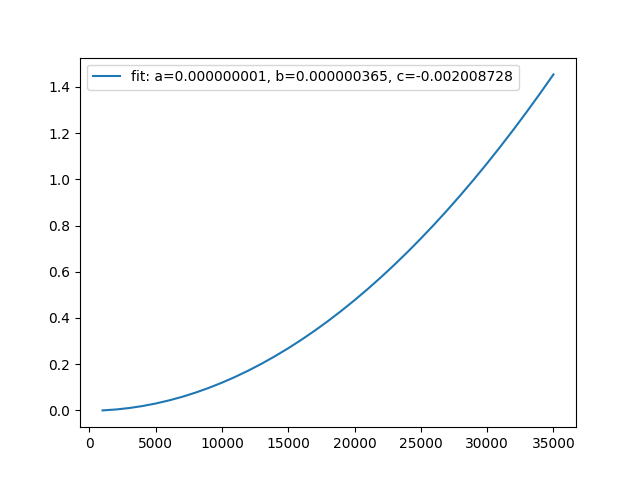
\includegraphics[width=.4\textwidth]{../graficos/insercion/insercion_elena.png}
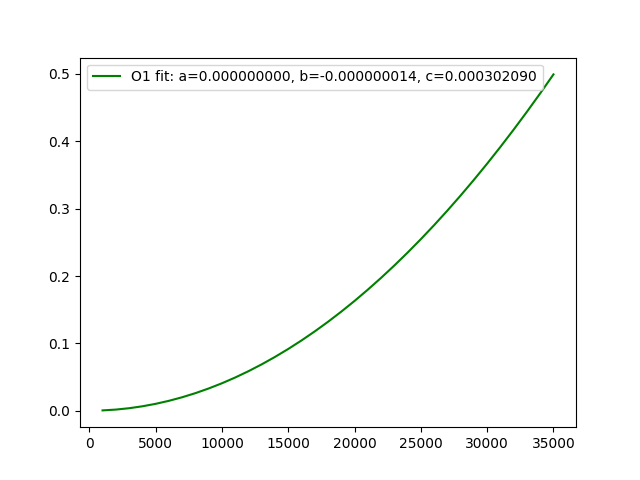
\includegraphics[width=.4\textwidth]{../graficos/insercion/insercion_O1_elena.png}
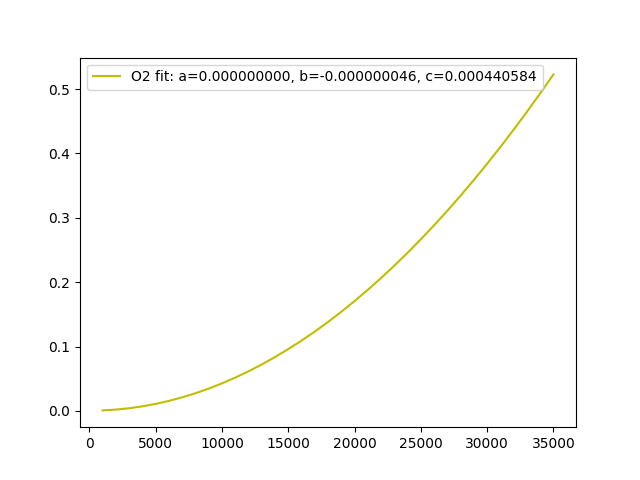
\includegraphics[width=.4\textwidth]{../graficos/insercion/insercion_O2_elena.png}
\end{center}
\begin{center}
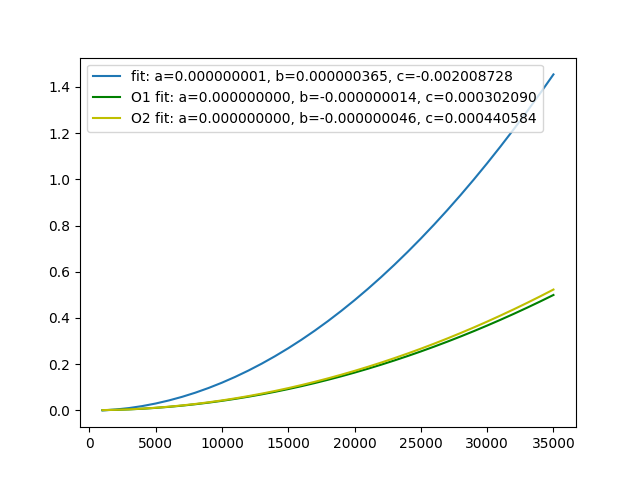
\includegraphics[width=.6\textwidth]{../graficos/insercion/insercion_juntas_elena.png}
\end{center}
\begin{center}
\begin{tabular}{| c | c | c | c |}
\hline
\textbf{N} & \textbf{O-} & \textbf{O1} & \textbf{O2} \\ \hline
1000 & 0.00128062 & 0.000394111 & 0.000471134 \\ \hline
2000 & 0.00494392 & 0.00164918 & 0.00169287 \\ \hline
3000 & 0.0107846 & 0.00370318 & 0.00386223 \\ \hline
4000 & 0.0190363 & 0.00655303 & 0.00742284 \\ \hline
5000 & 0.0290049 & 0.0104249 & 0.0111018 \\ \hline
6000 & 0.0417463 & 0.0149241 & 0.0154514 \\ \hline
7000 & 0.056829 & 0.0203957 & 0.0210657 \\ \hline
8000 & 0.074506 & 0.0262846 & 0.0275941 \\ \hline
9000 & 0.0937439 & 0.0331596 & 0.0347036 \\ \hline
10000 & 0.120899 & 0.0413018 & 0.0427021 \\ \hline
11000 & 0.146712 & 0.049628 & 0.05191 \\ \hline
12000 & 0.16882 & 0.0588039 & 0.0618677 \\ \hline
13000 & 0.197715 & 0.0691303 & 0.0729195 \\ \hline
14000 & 0.229951 & 0.0795406 & 0.0822059 \\ \hline
15000 & 0.266283 & 0.0931013 & 0.0958826 \\ \hline
16000 & 0.308386 & 0.105894 & 0.109572 \\ \hline
17000 & 0.339635 & 0.118275 & 0.123054 \\ \hline
18000 & 0.395265 & 0.131365 & 0.13857 \\ \hline
19000 & 0.430017 & 0.146577 & 0.154501 \\ \hline
20000 & 0.472572 & 0.163316 & 0.172057 \\ \hline
21000 & 0.520983 & 0.180018 & 0.192359 \\ \hline
22000 & 0.577108 & 0.200415 & 0.204682 \\ \hline
23000 & 0.661747 & 0.215635 & 0.224426 \\ \hline
24000 & 0.699163 & 0.234647 & 0.244675 \\ \hline
25000 & 0.745969 & 0.252221 & 0.270063 \\ \hline
26000 & 0.790776 & 0.277755 & 0.285303 \\ \hline
27000 & 0.85076 & 0.294963 & 0.308426 \\ \hline
28000 & 0.936871 & 0.315499 & 0.33406 \\ \hline
29000 & 1.0011 & 0.341928 & 0.357148 \\ \hline
30000 & 1.06186 & 0.365663 & 0.382002 \\ \hline
31000 & 1.14096 & 0.389944 & 0.411422 \\ \hline
32000 & 1.20885 & 0.424888 & 0.43873 \\ \hline
33000 & 1.28216 & 0.441153 & 0.46848 \\ \hline
34000 & 1.3752 & 0.475582 & 0.488904 \\ \hline
35000 & 1.47001 & 0.497147 & 0.52555 \\ \hline
\hline
\end{tabular}
\end{center}

\newpage
\subsection{Algoritmo insercion(Antonio)}
\begin{center}
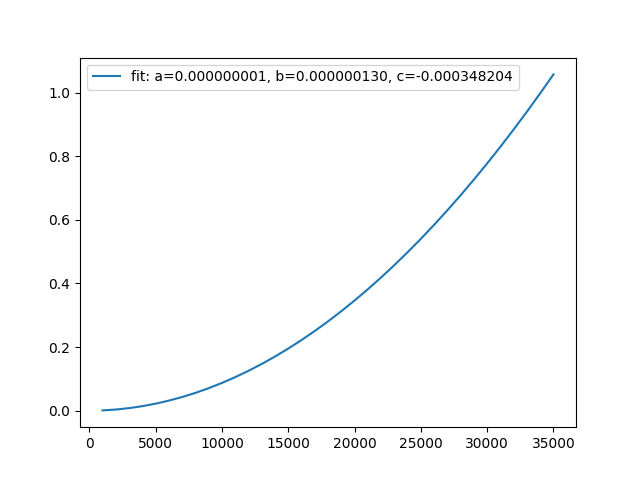
\includegraphics[width=.4\textwidth]{../graficos/insercion/insercion_antonio.png}
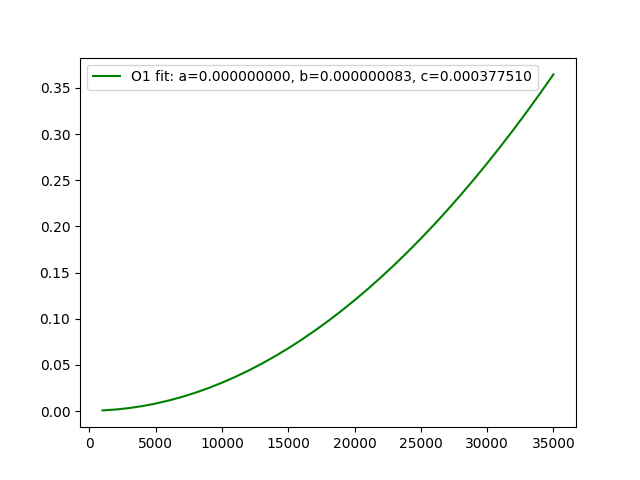
\includegraphics[width=.4\textwidth]{../graficos/insercion/insercion_O1_antonio.png}
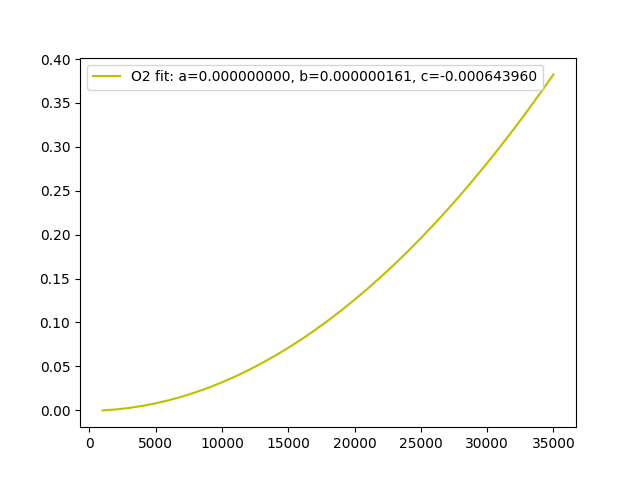
\includegraphics[width=.4\textwidth]{../graficos/insercion/insercion_O2_antonio.png}
\end{center}
\begin{center}
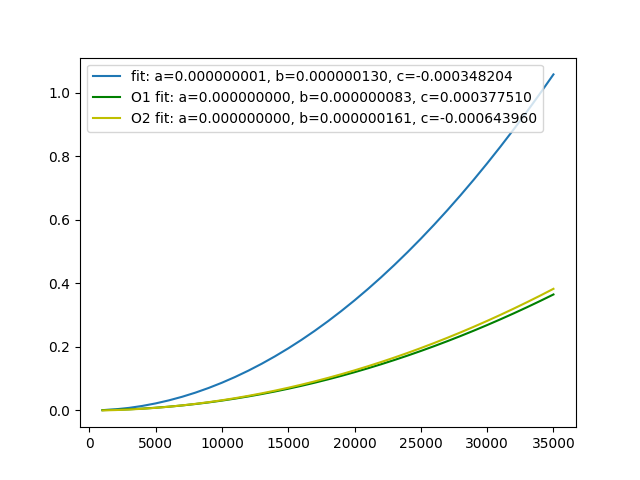
\includegraphics[width=.6\textwidth]{../graficos/insercion/insercion_juntas_antonio.png}
\end{center}
\begin{center}
\begin{tabular}{| c | c | c | c |}
\hline
\textbf{N} & \textbf{O-} & \textbf{O1} & \textbf{O2} \\ \hline
1000 & 0.0008668 & 0.000303425 & 0.000311528 \\ \hline
2000 & 0.00341429 & 0.00118489 & 0.00119304 \\ \hline
3000 & 0.00796838 & 0.00273074 & 0.00288727 \\ \hline
4000 & 0.0144405 & 0.00495307 & 0.00499236 \\ \hline
5000 & 0.021806 & 0.00779367 & 0.00801092 \\ \hline
6000 & 0.0316326 & 0.0111679 & 0.0112941 \\ \hline
7000 & 0.0426453 & 0.015719 & 0.0154039 \\ \hline
8000 & 0.0556216 & 0.0203325 & 0.0201064 \\ \hline
9000 & 0.0702031 & 0.0250042 & 0.0253493 \\ \hline
10000 & 0.0864261 & 0.0334055 & 0.0316306 \\ \hline
11000 & 0.105371 & 0.0371124 & 0.0379618 \\ \hline
12000 & 0.12481 & 0.0437312 & 0.044747 \\ \hline
13000 & 0.147354 & 0.0531294 & 0.0528693 \\ \hline
14000 & 0.169738 & 0.0605292 & 0.0612958 \\ \hline
15000 & 0.195663 & 0.0678626 & 0.0703497 \\ \hline
16000 & 0.22287 & 0.0775122 & 0.0801611 \\ \hline
17000 & 0.248004 & 0.0857529 & 0.0916148 \\ \hline
18000 & 0.276891 & 0.0973823 & 0.102555 \\ \hline
19000 & 0.310587 & 0.108259 & 0.115199 \\ \hline
20000 & 0.346986 & 0.119829 & 0.127033 \\ \hline
21000 & 0.383003 & 0.131816 & 0.139442 \\ \hline
22000 & 0.420818 & 0.144409 & 0.152354 \\ \hline
23000 & 0.457508 & 0.158134 & 0.166343 \\ \hline
24000 & 0.496786 & 0.172642 & 0.181194 \\ \hline
25000 & 0.538522 & 0.185073 & 0.199013 \\ \hline
26000 & 0.585611 & 0.201248 & 0.211649 \\ \hline
27000 & 0.627596 & 0.21768 & 0.227843 \\ \hline
28000 & 0.675989 & 0.236125 & 0.245768 \\ \hline
29000 & 0.728514 & 0.249836 & 0.26064 \\ \hline
30000 & 0.777847 & 0.267376 & 0.279988 \\ \hline
31000 & 0.829541 & 0.284786 & 0.299098 \\ \hline
32000 & 0.891975 & 0.305774 & 0.317623 \\ \hline
33000 & 0.945496 & 0.324868 & 0.341622 \\ \hline
34000 & 0.99809 & 0.344282 & 0.361573 \\ \hline
35000 & 1.04677 & 0.366523 & 0.384241 \\ \hline
\hline
\end{tabular}
\end{center}


\newpage
\subsection{Algoritmo seleccion(Elena)}
\begin{center}
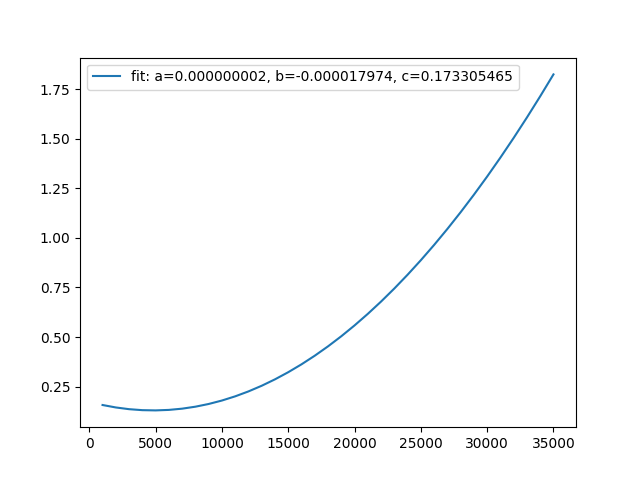
\includegraphics[width=.4\textwidth]{../graficos/seleccion/seleccion_elena.png}
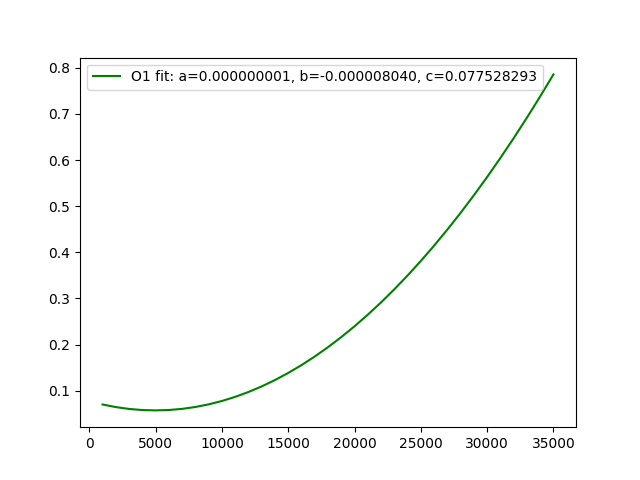
\includegraphics[width=.4\textwidth]{../graficos/seleccion/seleccion_O1_elena.png}
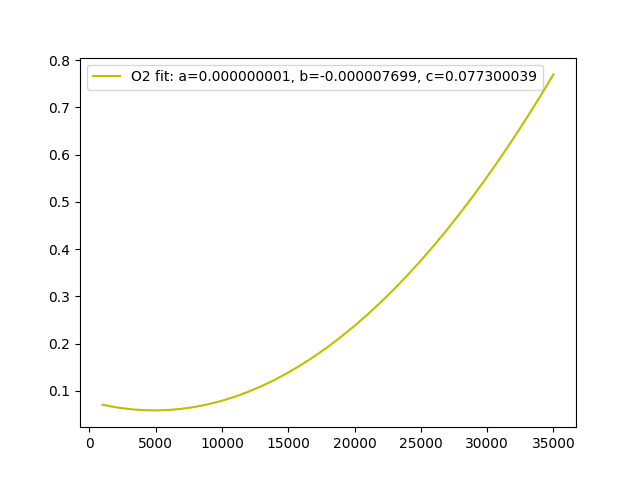
\includegraphics[width=.4\textwidth]{../graficos/seleccion/seleccion_O2_elena.png}
\end{center}
\begin{center}
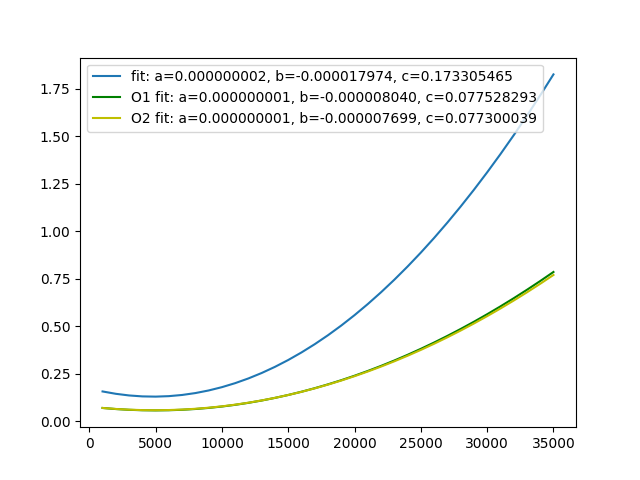
\includegraphics[width=.6\textwidth]{../graficos/seleccion/seleccion_juntas_elena.png}
\end{center}
\begin{center}
\begin{tabular}{| c | c | c | c |}
\hline
\textbf{N} & \textbf{O-} & \textbf{O1} & \textbf{O2} \\ \hline
1000 & 0.153329 & 0.0689078 & 0.0701804 \\ \hline
2000 & 0.600164 & 0.26289 & 0.26924 \\ \hline
3000 & 0.01341 & 0.00584541 & 0.00596033 \\ \hline
4000 & 0.0234943 & 0.0102879 & 0.0107875 \\ \hline
5000 & 0.0371377 & 0.016987 & 0.0159352 \\ \hline
6000 & 0.0532939 & 0.0253317 & 0.02325 \\ \hline
7000 & 0.0719599 & 0.0312657 & 0.0323246 \\ \hline
8000 & 0.094446 & 0.0413923 & 0.0404254 \\ \hline
9000 & 0.118314 & 0.0536091 & 0.0524062 \\ \hline
10000 & 0.150984 & 0.0648981 & 0.0645619 \\ \hline
11000 & 0.176848 & 0.0763845 & 0.0794243 \\ \hline
12000 & 0.20946 & 0.09047 & 0.0926502 \\ \hline
13000 & 0.247244 & 0.106174 & 0.106671 \\ \hline
14000 & 0.28852 & 0.122478 & 0.123979 \\ \hline
15000 & 0.328321 & 0.140205 & 0.136617 \\ \hline
16000 & 0.373965 & 0.159223 & 0.158134 \\ \hline
17000 & 0.42646 & 0.182532 & 0.179374 \\ \hline
18000 & 0.470287 & 0.209179 & 0.205501 \\ \hline
19000 & 0.526928 & 0.224175 & 0.226953 \\ \hline
20000 & 0.581037 & 0.250155 & 0.246477 \\ \hline
21000 & 0.643472 & 0.276663 & 0.273648 \\ \hline
22000 & 0.707557 & 0.308111 & 0.310535 \\ \hline
23000 & 0.769712 & 0.329961 & 0.321693 \\ \hline
24000 & 0.839798 & 0.36345 & 0.355474 \\ \hline
25000 & 0.909453 & 0.391991 & 0.387178 \\ \hline
26000 & 0.98656 & 0.422566 & 0.412706 \\ \hline
27000 & 1.06781 & 0.460135 & 0.461601 \\ \hline
28000 & 1.14912 & 0.48845 & 0.478346 \\ \hline
29000 & 1.23083 & 0.526664 & 0.52504 \\ \hline
30000 & 1.31034 & 0.559554 & 0.547864 \\ \hline
31000 & 1.39459 & 0.601733 & 0.589723 \\ \hline
32000 & 1.49614 & 0.645822 & 0.630297 \\ \hline
33000 & 1.58592 & 0.673679 & 0.670126 \\ \hline
34000 & 1.6822 & 0.72405 & 0.712463 \\ \hline
35000 & 1.78059 & 0.775574 & 0.747486 \\ \hline
\hline
\end{tabular}
\end{center}

\newpage
\subsection{Algoritmo seleccion(Antonio)}
\begin{center}
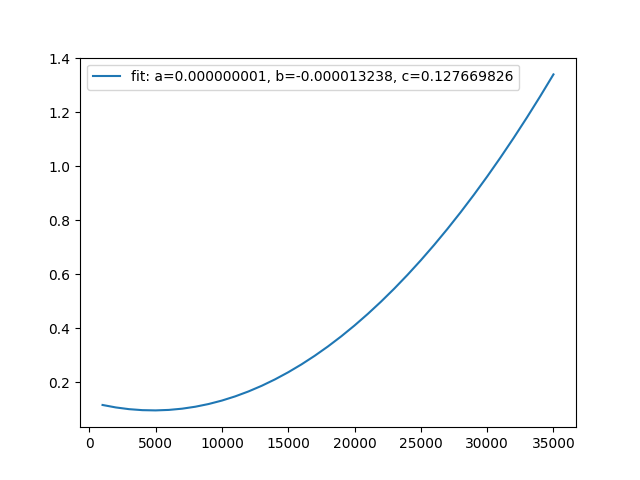
\includegraphics[width=.4\textwidth]{../graficos/seleccion/seleccion_antonio.png}
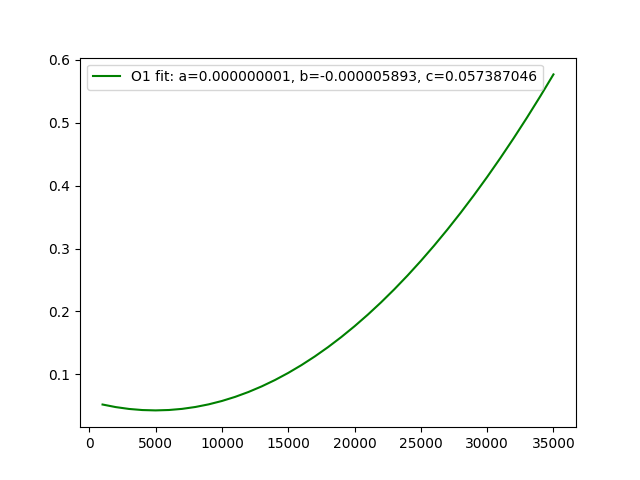
\includegraphics[width=.4\textwidth]{../graficos/seleccion/seleccion_O1_antonio.png}
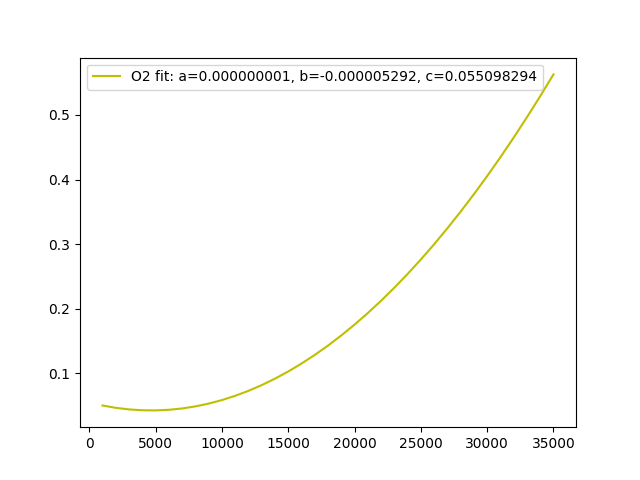
\includegraphics[width=.4\textwidth]{../graficos/seleccion/seleccion_O2_antonio.png}
\end{center}
\begin{center}
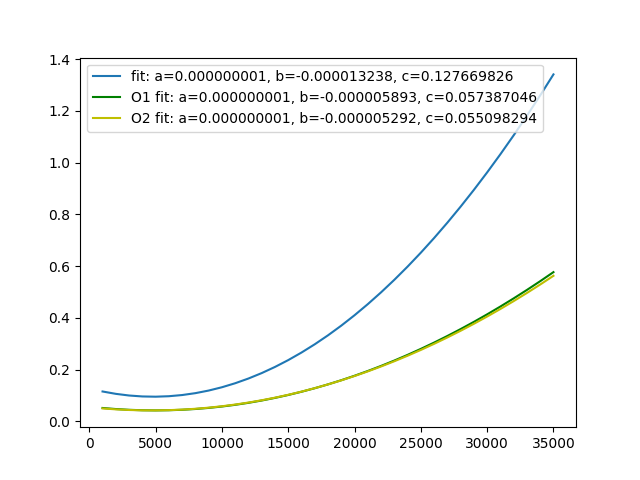
\includegraphics[width=.6\textwidth]{../graficos/seleccion/seleccion_juntas_antonio.png}
\end{center}
\begin{center}
\begin{tabular}{| c | c | c | c |}
\hline
\textbf{N} & \textbf{O-} & \textbf{O1} & \textbf{O2} \\ \hline
1000 & 0.113808 & 0.0507492 & 0.0515542 \\ \hline
2000 & 0.440022 & 0.194921 & 0.192643 \\ \hline
3000 & 0.00994115 & 0.00427214 & 0.00442329 \\ \hline
4000 & 0.0175305 & 0.00771941 & 0.00797904 \\ \hline
5000 & 0.0273612 & 0.0121969 & 0.0124481 \\ \hline
6000 & 0.0392684 & 0.0180733 & 0.0171079 \\ \hline
7000 & 0.0530349 & 0.0247544 & 0.0235386 \\ \hline
8000 & 0.0696024 & 0.0304388 & 0.0303601 \\ \hline
9000 & 0.0872593 & 0.0399728 & 0.0385527 \\ \hline
10000 & 0.108057 & 0.0471915 & 0.0476896 \\ \hline
11000 & 0.13081 & 0.0563163 & 0.0637525 \\ \hline
12000 & 0.154417 & 0.0666793 & 0.0668392 \\ \hline
13000 & 0.181586 & 0.0784763 & 0.0771758 \\ \hline
14000 & 0.21108 & 0.0922109 & 0.090675 \\ \hline
15000 & 0.246563 & 0.105169 & 0.103795 \\ \hline
16000 & 0.274096 & 0.12036 & 0.117137 \\ \hline
17000 & 0.309675 & 0.135038 & 0.13268 \\ \hline
18000 & 0.346677 & 0.152715 & 0.15029 \\ \hline
19000 & 0.387027 & 0.166195 & 0.172956 \\ \hline
20000 & 0.428833 & 0.183288 & 0.191728 \\ \hline
21000 & 0.476191 & 0.204037 & 0.20652 \\ \hline
22000 & 0.518642 & 0.220613 & 0.221813 \\ \hline
23000 & 0.56802 & 0.243047 & 0.240955 \\ \hline
24000 & 0.618507 & 0.262949 & 0.258005 \\ \hline
25000 & 0.668424 & 0.284926 & 0.282445 \\ \hline
26000 & 0.72458 & 0.315597 & 0.30513 \\ \hline
27000 & 0.783398 & 0.333334 & 0.325479 \\ \hline
28000 & 0.838477 & 0.367546 & 0.351541 \\ \hline
29000 & 0.897708 & 0.390469 & 0.381924 \\ \hline
30000 & 0.964555 & 0.416259 & 0.408663 \\ \hline
31000 & 1.02975 & 0.43713 & 0.429654 \\ \hline
32000 & 1.09034 & 0.47207 & 0.455585 \\ \hline
33000 & 1.16999 & 0.493228 & 0.497087 \\ \hline
34000 & 1.23219 & 0.528135 & 0.518997 \\ \hline
35000 & 1.31538 & 0.573425 & 0.550583 \\ \hline
\hline
\end{tabular}
\end{center}


\newpage
\subsection{Algoritmo mergesort(Elena)}
\begin{center}
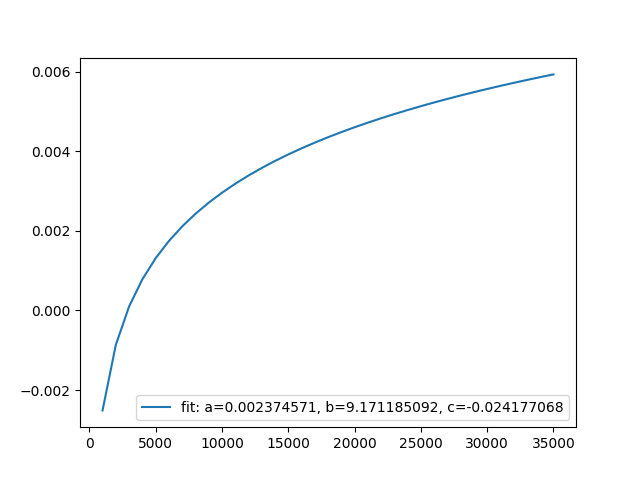
\includegraphics[width=.4\textwidth]{../graficos/mergesort/mergesort_elena.png}
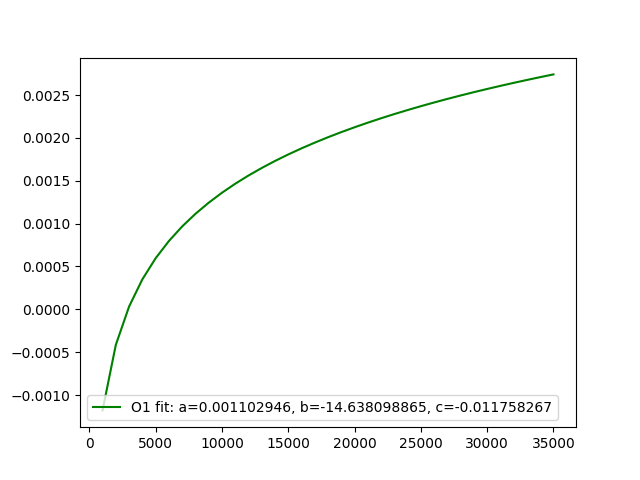
\includegraphics[width=.4\textwidth]{../graficos/mergesort/mergesort_O1_elena.png}
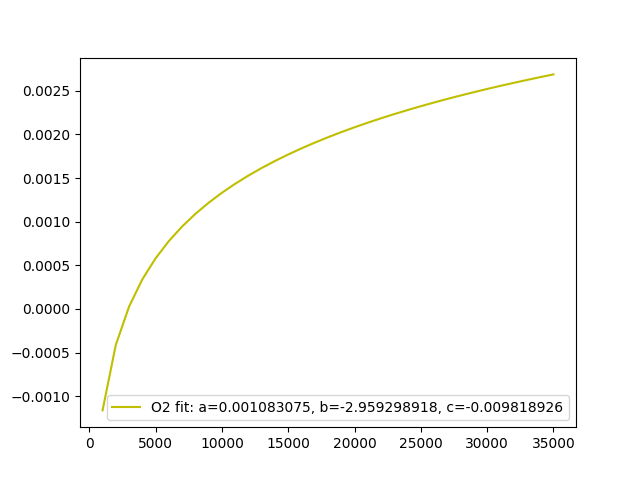
\includegraphics[width=.4\textwidth]{../graficos/mergesort/mergesort_O2_elena.png}
\end{center}
\begin{center}
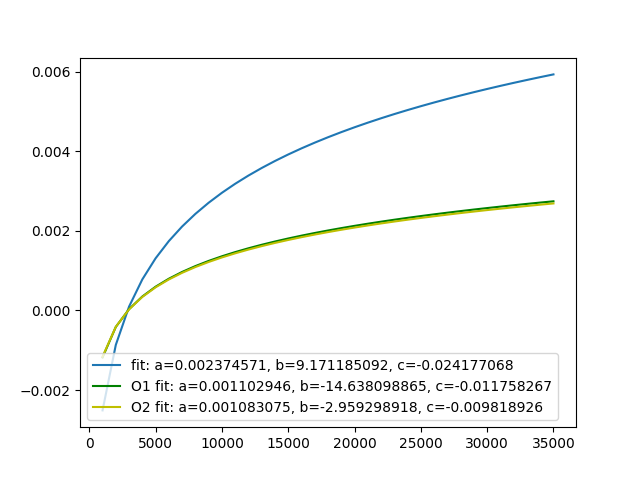
\includegraphics[width=.6\textwidth]{../graficos/mergesort/mergesort_juntas_elena.png}
\end{center}
\begin{center}
\begin{tabular}{| c | c | c | c |}
\hline
\textbf{N} & \textbf{O-} & \textbf{O1} & \textbf{O2} \\ \hline
1000 & 0.000142289 & 5.6138e-05 & 5.3256e-05 \\ \hline
2000 & 0.000301 & 0.00014214 & 0.000129577 \\ \hline
3000 & 0.000565186 & 0.000238601 & 0.000234651 \\ \hline
4000 & 0.000656325 & 0.000291011 & 0.000289394 \\ \hline
5000 & 0.000912161 & 0.000394628 & 0.000390957 \\ \hline
6000 & 0.00120506 & 0.000520647 & 0.000514568 \\ \hline
7000 & 0.00117797 & 0.000533973 & 0.00051628 \\ \hline
8000 & 0.00141341 & 0.000645499 & 0.000621247 \\ \hline
9000 & 0.00168161 & 0.000752588 & 0.00073346 \\ \hline
10000 & 0.00196429 & 0.000865177 & 0.000849189 \\ \hline
11000 & 0.002299 & 0.000993 & 0.001001 \\ \hline
12000 & 0.002597 & 0.001195 & 0.001114 \\ \hline
13000 & 0.002363 & 0.001145 & 0.001098 \\ \hline
14000 & 0.002612 & 0.001259 & 0.001197 \\ \hline
15000 & 0.002866 & 0.00136 & 0.001286 \\ \hline
16000 & 0.003107 & 0.001472 & 0.001672 \\ \hline
17000 & 0.00342 & 0.001594 & 0.001538 \\ \hline
18000 & 0.00364 & 0.001705 & 0.001687 \\ \hline
19000 & 0.003965 & 0.001841 & 0.001756 \\ \hline
20000 & 0.004258 & 0.001948 & 0.001864 \\ \hline
21000 & 0.004619 & 0.002085 & 0.002014 \\ \hline
22000 & 0.004883 & 0.002211 & 0.002173 \\ \hline
23000 & 0.005268 & 0.002372 & 0.002323 \\ \hline
24000 & 0.005586 & 0.002533 & 0.002458 \\ \hline
25000 & 0.005926 & 0.002623 & 0.00259 \\ \hline
26000 & 0.00509 & 0.002435 & 0.002348 \\ \hline
27000 & 0.005307 & 0.002543 & 0.002464 \\ \hline
28000 & 0.005557 & 0.002629 & 0.002535 \\ \hline
29000 & 0.005838 & 0.002783 & 0.002755 \\ \hline
30000 & 0.006091 & 0.002903 & 0.002788 \\ \hline
31000 & 0.006358 & 0.00301 & 0.003131 \\ \hline
32000 & 0.006704 & 0.003126 & 0.003015 \\ \hline
33000 & 0.006881 & 0.003241 & 0.003203 \\ \hline
34000 & 0.007221 & 0.003394 & 0.003348 \\ \hline
35000 & 0.008392 & 0.003499 & 0.003422 \\ \hline
\hline
\end{tabular}
\end{center}

\newpage
\subsection{Algoritmo mergesort(Antonio)}
\begin{center}
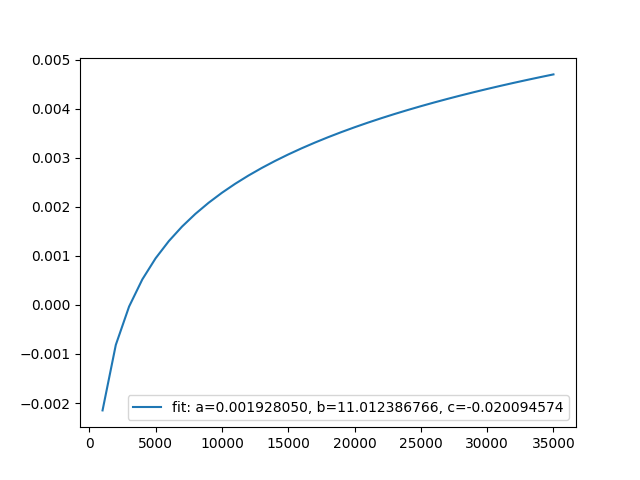
\includegraphics[width=.4\textwidth]{../graficos/mergesort/mergesort_antonio.png}
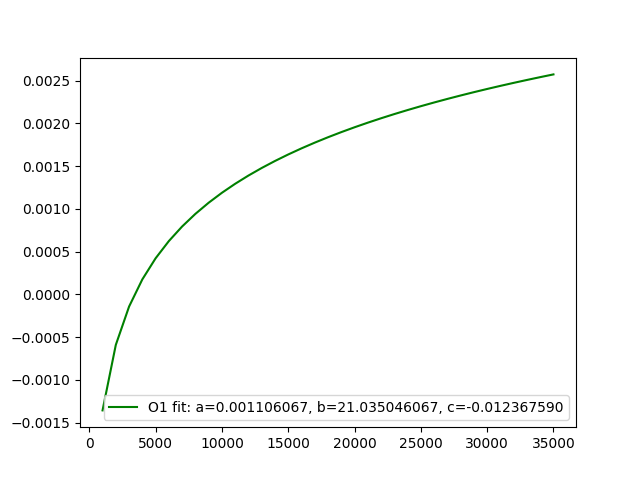
\includegraphics[width=.4\textwidth]{../graficos/mergesort/mergesort_O1_antonio.png}
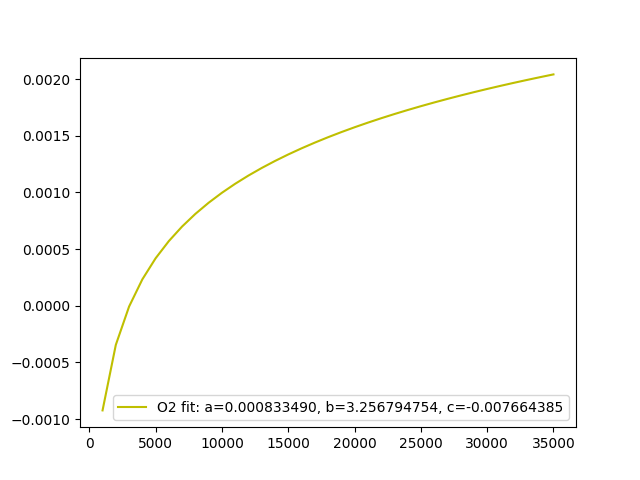
\includegraphics[width=.4\textwidth]{../graficos/mergesort/mergesort_O2_antonio.png}
\end{center}
\begin{center}
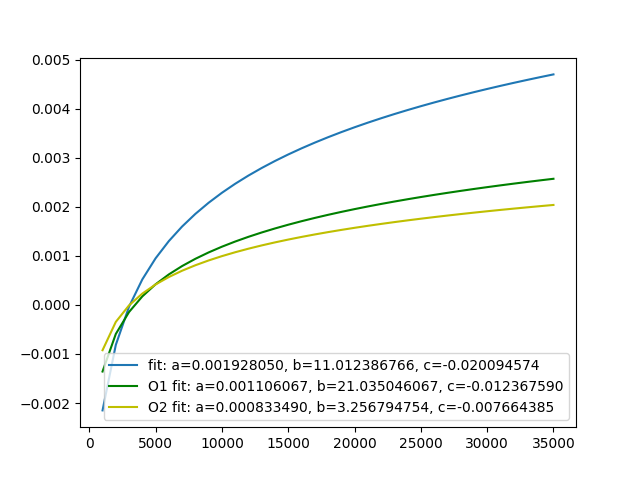
\includegraphics[width=.6\textwidth]{../graficos/mergesort/mergesort_juntas_antonio.png}
\end{center}
\begin{center}
\begin{tabular}{| c | c | c | c |}
\hline
\textbf{N} & \textbf{O-} & \textbf{O1} & \textbf{O2} \\ \hline
1000 & 9.7562e-05 & 4.3121e-05 & 5.0206e-05 \\ \hline
2000 & 0.000219378 & 9.4759e-05 & 9.4657e-05 \\ \hline
3000 & 0.00040376 & 0.000172173 & 0.000173778 \\ \hline
4000 & 0.000478964 & 0.000214573 & 0.00021195 \\ \hline
5000 & 0.000672422 & 0.000290972 & 0.000283667 \\ \hline
6000 & 0.000882371 & 0.000376491 & 0.000377717 \\ \hline
7000 & 0.000861508 & 0.000395036 & 0.000384458 \\ \hline
8000 & 0.00102842 & 0.000473047 & 0.000454253 \\ \hline
9000 & 0.00124205 & 0.000547581 & 0.000538787 \\ \hline
10000 & 0.00141724 & 0.00063134 & 0.000612704 \\ \hline
11000 & 0.001626 & 0.000733 & 0.000785 \\ \hline
12000 & 0.001873 & 0.00083 & 0.000817 \\ \hline
13000 & 0.001741 & 0.000866 & 0.00077 \\ \hline
14000 & 0.001882 & 0.000877 & 0.000853 \\ \hline
15000 & 0.002088 & 0.001076 & 0.000928 \\ \hline
16000 & 0.002283 & 0.001159 & 0.001068 \\ \hline
17000 & 0.002514 & 0.001251 & 0.001073 \\ \hline
18000 & 0.002668 & 0.001347 & 0.001173 \\ \hline
19000 & 0.002942 & 0.001447 & 0.001405 \\ \hline
20000 & 0.003065 & 0.001693 & 0.001409 \\ \hline
21000 & 0.003437 & 0.001797 & 0.001555 \\ \hline
22000 & 0.003711 & 0.001916 & 0.001606 \\ \hline
23000 & 0.004279 & 0.002046 & 0.001739 \\ \hline
24000 & 0.004591 & 0.002171 & 0.001814 \\ \hline
25000 & 0.004832 & 0.002307 & 0.001987 \\ \hline
26000 & 0.00456 & 0.002109 & 0.00174 \\ \hline
27000 & 0.004326 & 0.00221 & 0.001877 \\ \hline
28000 & 0.004546 & 0.002307 & 0.001978 \\ \hline
29000 & 0.004755 & 0.002664 & 0.002051 \\ \hline
30000 & 0.004972 & 0.002788 & 0.002072 \\ \hline
31000 & 0.005207 & 0.003251 & 0.00222 \\ \hline
32000 & 0.00544 & 0.003364 & 0.002253 \\ \hline
33000 & 0.005668 & 0.003491 & 0.002364 \\ \hline
34000 & 0.005887 & 0.003664 & 0.002718 \\ \hline
35000 & 0.006174 & 0.003781 & 0.003063 \\ \hline
\hline
\end{tabular}
\end{center}


\newpage
\subsection{Algoritmo quicksort(Elena)}
\begin{center}
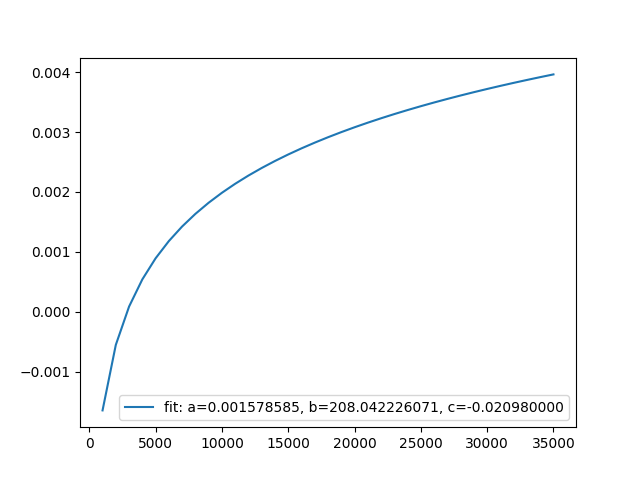
\includegraphics[width=.4\textwidth]{../graficos/quicksort/quicksort_elena.png}
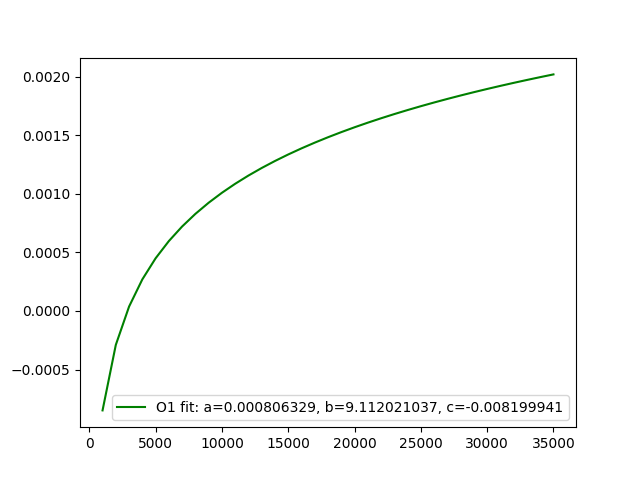
\includegraphics[width=.4\textwidth]{../graficos/quicksort/quicksort_O1_elena.png}
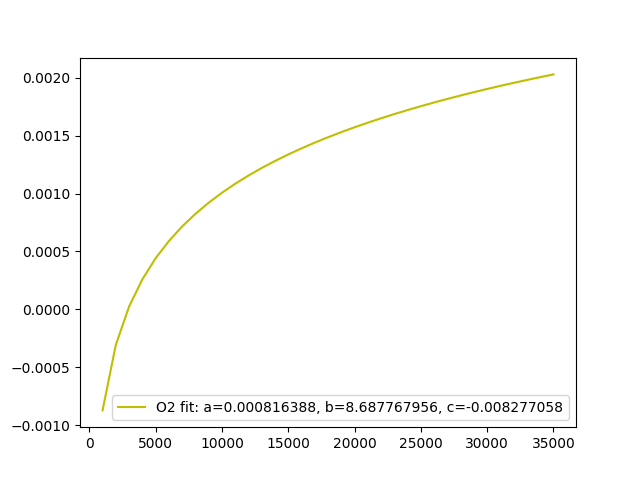
\includegraphics[width=.4\textwidth]{../graficos/quicksort/quicksort_O2_elena.png}
\end{center}
\begin{center}
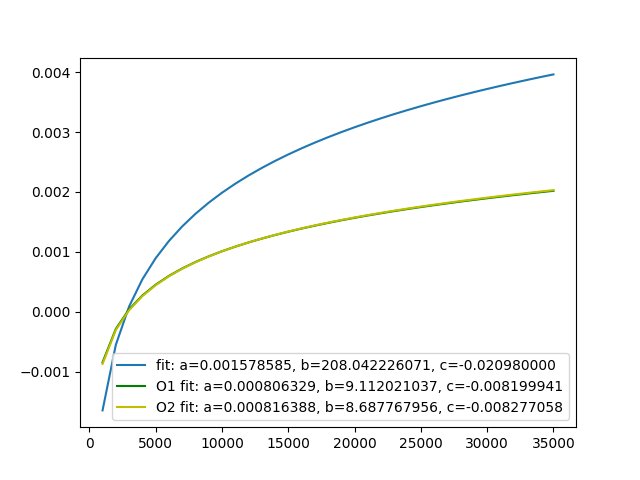
\includegraphics[width=.6\textwidth]{../graficos/quicksort/quicksort_juntas_elena.png}
\end{center}
\begin{center}
\begin{tabular}{| c | c | c | c |}
\hline
\textbf{N} & \textbf{O-} & \textbf{O1} & \textbf{O2} \\ \hline
1000 & 9.9817e-05 & 5.0442e-05 & 5.0401e-05 \\ \hline
2000 & 0.000227257 & 0.00013266 & 0.000118967 \\ \hline
3000 & 0.000350887 & 0.00017088 & 0.000175812 \\ \hline
4000 & 0.000482895 & 0.00023387 & 0.00023271 \\ \hline
5000 & 0.000646748 & 0.000302824 & 0.000304232 \\ \hline
6000 & 0.000749643 & 0.000374281 & 0.000369755 \\ \hline
7000 & 0.000908375 & 0.00044219 & 0.000437503 \\ \hline
8000 & 0.00105866 & 0.000523946 & 0.000509061 \\ \hline
9000 & 0.00117842 & 0.000585779 & 0.000581393 \\ \hline
10000 & 0.00132631 & 0.000658304 & 0.000652338 \\ \hline
11000 & 0.00145902 & 0.000734204 & 0.000726409 \\ \hline
12000 & 0.00166884 & 0.000809363 & 0.00080204 \\ \hline
13000 & 0.00169378 & 0.000844834 & 0.000853763 \\ \hline
14000 & 0.00186206 & 0.00106827 & 0.000932916 \\ \hline
15000 & 0.0019978 & 0.00101793 & 0.00100616 \\ \hline
16000 & 0.00219878 & 0.0011337 & 0.00108273 \\ \hline
17000 & 0.00232444 & 0.0012006 & 0.00119566 \\ \hline
18000 & 0.00244827 & 0.0012454 & 0.00124138 \\ \hline
19000 & 0.00258529 & 0.00131713 & 0.00130758 \\ \hline
20000 & 0.00272364 & 0.00139903 & 0.00138977 \\ \hline
21000 & 0.00299948 & 0.00146522 & 0.00147639 \\ \hline
22000 & 0.00303522 & 0.00155317 & 0.0015648 \\ \hline
23000 & 0.00319398 & 0.00158218 & 0.0016267 \\ \hline
24000 & 0.00330492 & 0.00172188 & 0.00175563 \\ \hline
25000 & 0.00351289 & 0.00179055 & 0.00186384 \\ \hline
26000 & 0.00368799 & 0.0018612 & 0.0018534 \\ \hline
27000 & 0.00382549 & 0.00194992 & 0.00200636 \\ \hline
28000 & 0.00397248 & 0.00200078 & 0.00203078 \\ \hline
29000 & 0.00418752 & 0.00210934 & 0.00210808 \\ \hline
30000 & 0.00429072 & 0.002219 & 0.00222609 \\ \hline
31000 & 0.00438885 & 0.00224658 & 0.0022822 \\ \hline
32000 & 0.00453243 & 0.00237256 & 0.00237227 \\ \hline
33000 & 0.0048428 & 0.0024454 & 0.00241964 \\ \hline
34000 & 0.00491766 & 0.00248939 & 0.00255495 \\ \hline
35000 & 0.00503133 & 0.00254678 & 0.00256313 \\ \hline
\hline
\end{tabular}
\end{center}

\newpage
\subsection{Algoritmo quicksort(Antonio)}
\begin{center}
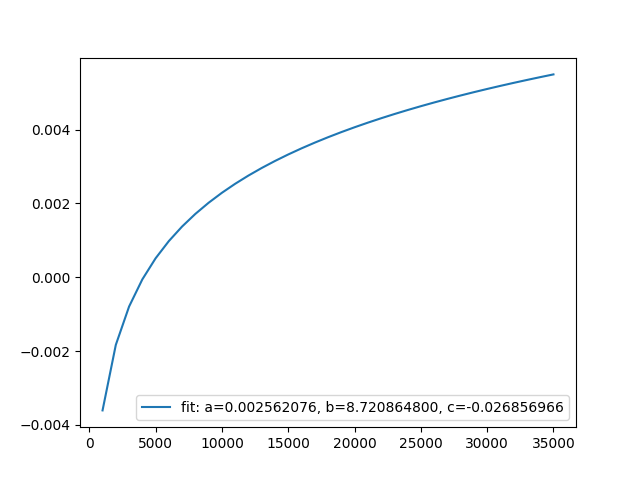
\includegraphics[width=.4\textwidth]{../graficos/quicksort/quicksort_antonio.png}
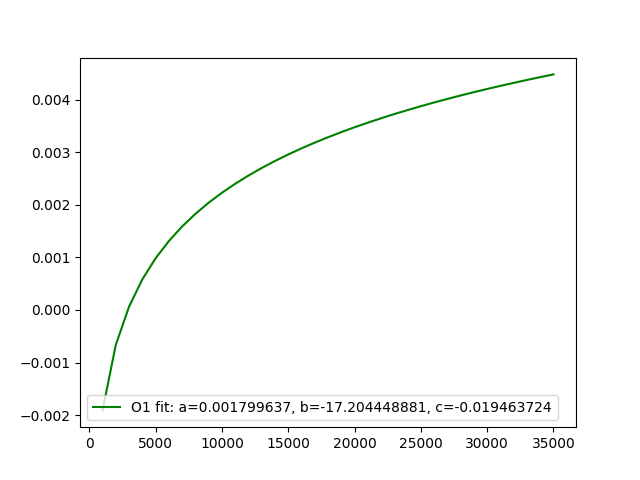
\includegraphics[width=.4\textwidth]{../graficos/quicksort/quicksort_O1_antonio.png}
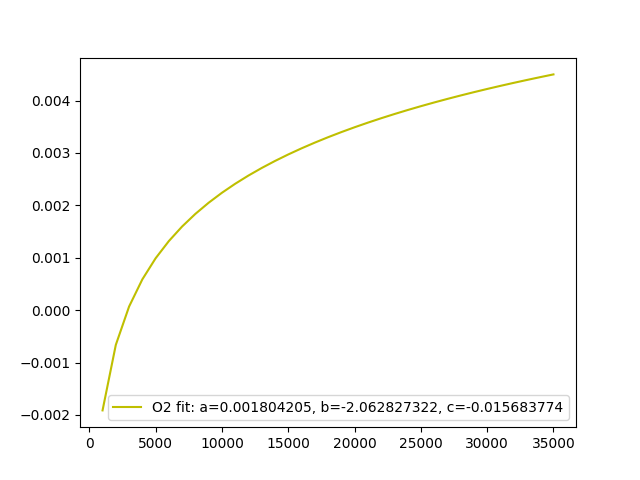
\includegraphics[width=.4\textwidth]{../graficos/quicksort/quicksort_O2_antonio.png}
\end{center}
\begin{center}
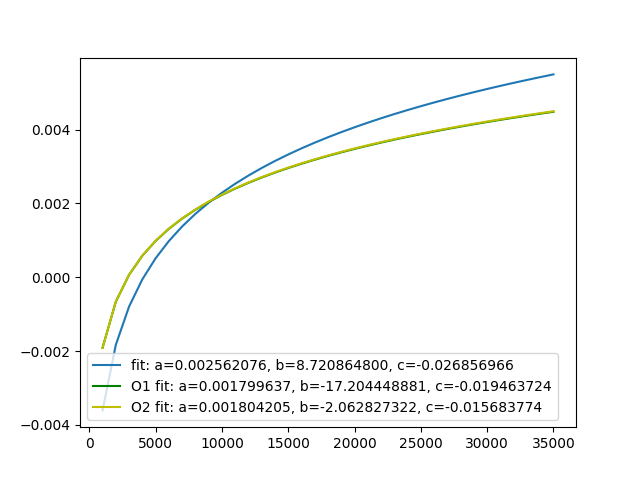
\includegraphics[width=.6\textwidth]{../graficos/quicksort/quicksort_juntas_antonio.png}
\end{center}
\begin{center}
\begin{tabular}{| c | c | c | c |}
\hline
\textbf{N} & \textbf{O-} & \textbf{O1} & \textbf{O2} \\ \hline
1000 & 7.0852e-05 & 8.7531e-05 & 0.000113581 \\ \hline
2000 & 0.00021565 & 0.000199469 & 0.000243369 \\ \hline
3000 & 0.000242762 & 0.000305245 & 0.00038559 \\ \hline
4000 & 0.000328305 & 0.000526492 & 0.000535741 \\ \hline
5000 & 0.000426144 & 0.000659839 & 0.0006694 \\ \hline
6000 & 0.000523048 & 0.000837415 & 0.000817214 \\ \hline
7000 & 0.000616916 & 0.000965552 & 0.0009916 \\ \hline
8000 & 0.000780271 & 0.0012482 & 0.00115136 \\ \hline
9000 & 0.000803905 & 0.00129618 & 0.00130735 \\ \hline
10000 & 0.000947855 & 0.00153631 & 0.00148174 \\ \hline
11000 & 0.00108127 & 0.00172348 & 0.00162444 \\ \hline
12000 & 0.00112693 & 0.00186451 & 0.00179318 \\ \hline
13000 & 0.00131472 & 0.00195875 & 0.0019322 \\ \hline
14000 & 0.00144836 & 0.00210791 & 0.00213215 \\ \hline
15000 & 0.00157483 & 0.00233087 & 0.00226752 \\ \hline
16000 & 0.00166702 & 0.00239326 & 0.00246252 \\ \hline
17000 & 0.00170516 & 0.00257679 & 0.00264973 \\ \hline
18000 & 0.00203383 & 0.00276208 & 0.00276352 \\ \hline
19000 & 0.00213518 & 0.00305852 & 0.00295137 \\ \hline
20000 & 0.00223099 & 0.00304744 & 0.0031493 \\ \hline
21000 & 0.00235415 & 0.00329863 & 0.00330143 \\ \hline
22000 & 0.00245928 & 0.00355411 & 0.00351015 \\ \hline
23000 & 0.00261111 & 0.00360215 & 0.00363866 \\ \hline
24000 & 0.0032673 & 0.00373966 & 0.00381169 \\ \hline
25000 & 0.00386305 & 0.00390432 & 0.00396249 \\ \hline
26000 & 0.00447933 & 0.00414109 & 0.00413046 \\ \hline
27000 & 0.0056785 & 0.00425661 & 0.00433613 \\ \hline
28000 & 0.00589681 & 0.00450222 & 0.00451823 \\ \hline
29000 & 0.00740397 & 0.00464354 & 0.00469539 \\ \hline
30000 & 0.00773386 & 0.00482171 & 0.00483742 \\ \hline
31000 & 0.00793326 & 0.0049767 & 0.00503622 \\ \hline
32000 & 0.00834004 & 0.00530646 & 0.0052259 \\ \hline
33000 & 0.00838877 & 0.00536436 & 0.0054252 \\ \hline
34000 & 0.00881353 & 0.00555759 & 0.00557981 \\ \hline
35000 & 0.00921185 & 0.00573696 & 0.00579729 \\ \hline
\hline
\end{tabular}
\end{center}


\newpage
\subsection{Algoritmo heapsort(Elena)}
\begin{center}
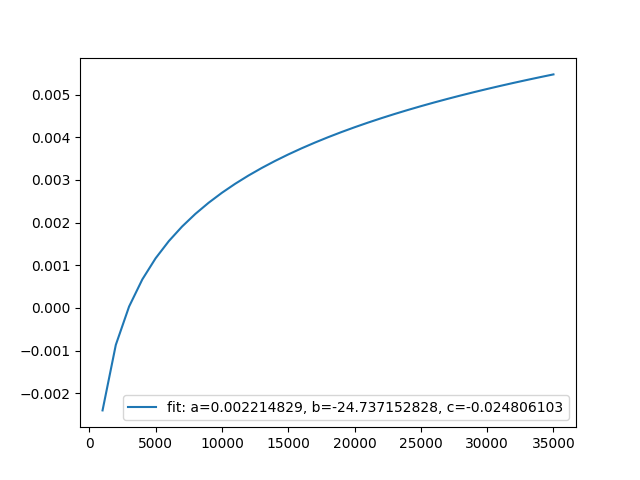
\includegraphics[width=.4\textwidth]{../graficos/heapsort/heapsort_elena.png}
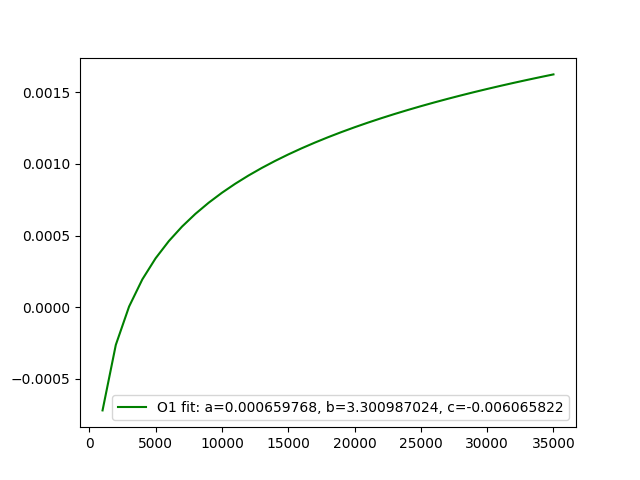
\includegraphics[width=.4\textwidth]{../graficos/heapsort/heapsort_O1_elena.png}
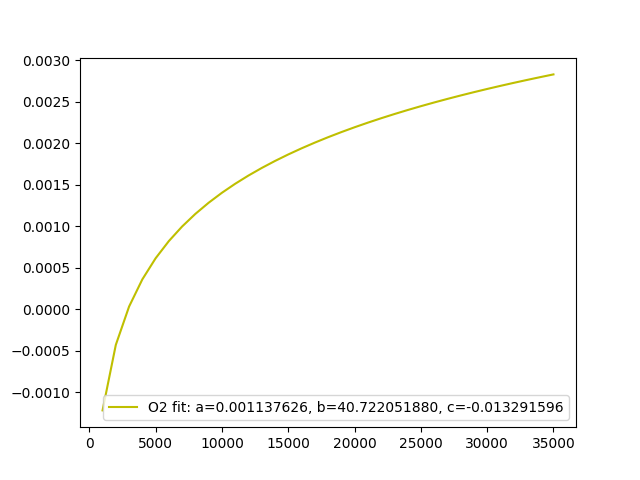
\includegraphics[width=.4\textwidth]{../graficos/heapsort/heapsort_O2_elena.png}
\end{center}
\begin{center}
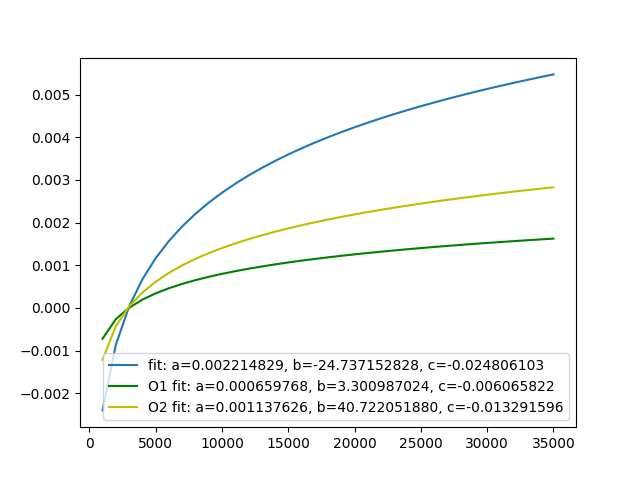
\includegraphics[width=.6\textwidth]{../graficos/heapsort/heapsort_juntas_elena.png}
\end{center}
\begin{center}
\begin{tabular}{| c | c | c | c |}
\hline
\textbf{N} & \textbf{O-} & \textbf{O1} & \textbf{O2} \\ \hline
1000 & 0.000136123 & 4.4751e-05 & 6.9021e-05 \\ \hline
2000 & 0.000306375 & 8.0885e-05 & 0.00015095 \\ \hline
3000 & 0.000452397 & 0.000128777 & 0.00023365 \\ \hline
4000 & 0.00061982 & 0.000181898 & 0.000326824 \\ \hline
5000 & 0.00080802 & 0.000229764 & 0.000416221 \\ \hline
6000 & 0.000970036 & 0.000276247 & 0.000507487 \\ \hline
7000 & 0.00114352 & 0.000337848 & 0.000636754 \\ \hline
8000 & 0.00134811 & 0.000390992 & 0.000704134 \\ \hline
9000 & 0.00154743 & 0.000448341 & 0.000804659 \\ \hline
10000 & 0.00172895 & 0.000503122 & 0.000924079 \\ \hline
11000 & 0.00192196 & 0.000550752 & 0.00102253 \\ \hline
12000 & 0.00212514 & 0.000622282 & 0.00110433 \\ \hline
13000 & 0.00233904 & 0.000685348 & 0.00120639 \\ \hline
14000 & 0.00249019 & 0.000742696 & 0.00131808 \\ \hline
15000 & 0.00277069 & 0.000802099 & 0.0014206 \\ \hline
16000 & 0.00289043 & 0.00088007 & 0.00152127 \\ \hline
17000 & 0.00318939 & 0.000929104 & 0.00164515 \\ \hline
18000 & 0.00330463 & 0.00097859 & 0.00175197 \\ \hline
19000 & 0.00350129 & 0.00103657 & 0.00184024 \\ \hline
20000 & 0.00370489 & 0.00111178 & 0.00196114 \\ \hline
21000 & 0.0038996 & 0.00119041 & 0.0020682 \\ \hline
22000 & 0.00416611 & 0.00126033 & 0.00217102 \\ \hline
23000 & 0.00432359 & 0.00129826 & 0.0023439 \\ \hline
24000 & 0.00454306 & 0.00136747 & 0.00237447 \\ \hline
25000 & 0.00483153 & 0.00143063 & 0.00250477 \\ \hline
26000 & 0.00497735 & 0.0014979 & 0.0026143 \\ \hline
27000 & 0.0052003 & 0.00156599 & 0.00272145 \\ \hline
28000 & 0.00545135 & 0.00163357 & 0.00285597 \\ \hline
29000 & 0.00554687 & 0.00169604 & 0.00294463 \\ \hline
30000 & 0.00572157 & 0.00177656 & 0.00306901 \\ \hline
31000 & 0.00594329 & 0.00186258 & 0.0031558 \\ \hline
32000 & 0.00790022 & 0.00188938 & 0.00330005 \\ \hline
33000 & 0.00660048 & 0.00199688 & 0.00340508 \\ \hline
34000 & 0.00675016 & 0.00202066 & 0.00352505 \\ \hline
35000 & 0.00688566 & 0.00212635 & 0.00362913 \\ \hline
\hline
\end{tabular}
\end{center}

\newpage
\subsection{Algoritmo heapsort(Antonio)}
\begin{center}
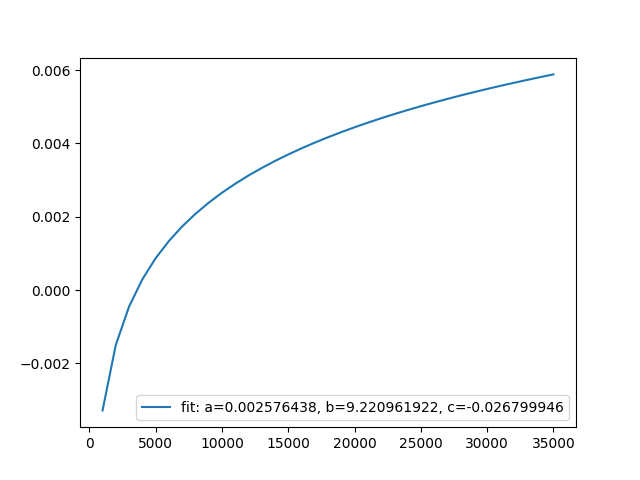
\includegraphics[width=.4\textwidth]{../graficos/heapsort/heapsort_antonio.png}
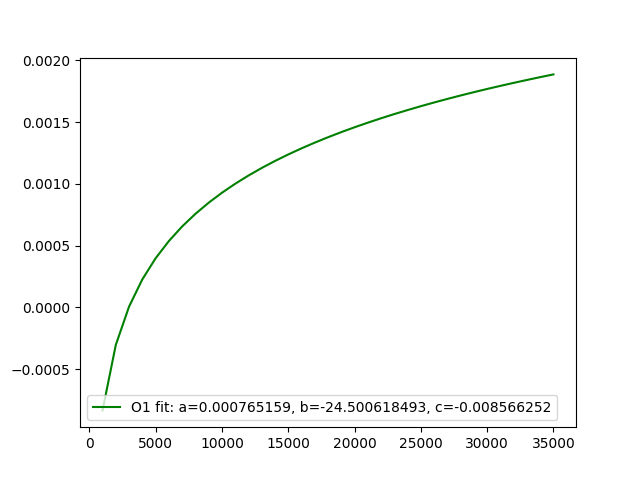
\includegraphics[width=.4\textwidth]{../graficos/heapsort/heapsort_O1_antonio.png}
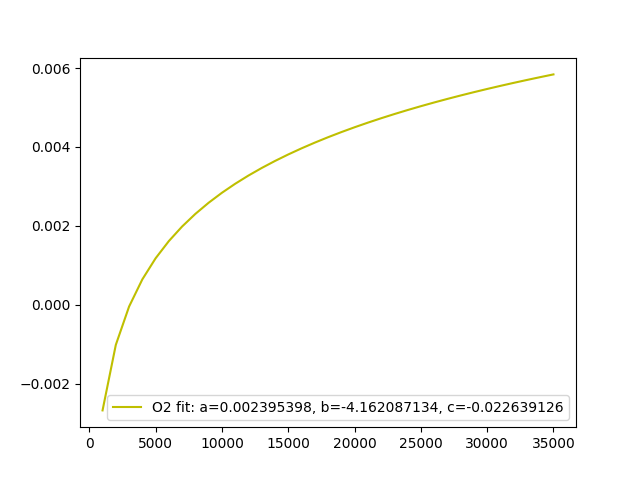
\includegraphics[width=.4\textwidth]{../graficos/heapsort/heapsort_O2_antonio.png}
\end{center}
\begin{center}
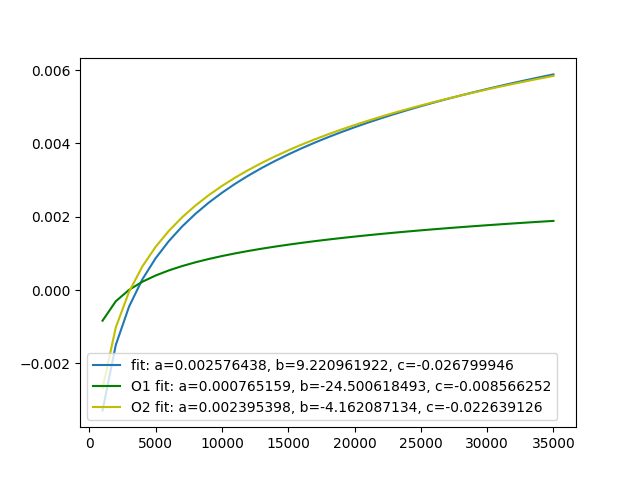
\includegraphics[width=.6\textwidth]{../graficos/heapsort/heapsort_juntas_antonio.png}
\end{center}
\begin{center}
\begin{tabular}{| c | c | c | c |}
\hline
\textbf{N} & \textbf{O-} & \textbf{O1} & \textbf{O2} \\ \hline
1000 & 9.5007e-05 & 4.4977e-05 & 8.2139e-05 \\ \hline
2000 & 0.000203424 & 9.8924e-05 & 0.000176791 \\ \hline
3000 & 0.000320315 & 0.000152058 & 0.000372852 \\ \hline
4000 & 0.000440649 & 0.000206437 & 0.000627335 \\ \hline
5000 & 0.00056368 & 0.000273043 & 0.000805891 \\ \hline
6000 & 0.00075261 & 0.000333338 & 0.000983016 \\ \hline
7000 & 0.000893066 & 0.000396277 & 0.00118707 \\ \hline
8000 & 0.00100186 & 0.000449124 & 0.00137798 \\ \hline
9000 & 0.00114237 & 0.000538101 & 0.00156823 \\ \hline
10000 & 0.00128021 & 0.00058067 & 0.00173922 \\ \hline
11000 & 0.00155514 & 0.000660495 & 0.00194511 \\ \hline
12000 & 0.00157578 & 0.000718106 & 0.00216217 \\ \hline
13000 & 0.00172319 & 0.000787455 & 0.00232897 \\ \hline
14000 & 0.00202401 & 0.000854124 & 0.00252672 \\ \hline
15000 & 0.00201206 & 0.000934659 & 0.00272894 \\ \hline
16000 & 0.00254391 & 0.00103014 & 0.00294308 \\ \hline
17000 & 0.00236532 & 0.00107292 & 0.00354848 \\ \hline
18000 & 0.00253443 & 0.00114383 & 0.00380026 \\ \hline
19000 & 0.00266495 & 0.00122477 & 0.00389984 \\ \hline
20000 & 0.00317532 & 0.00127798 & 0.00403938 \\ \hline
21000 & 0.00404545 & 0.00134584 & 0.00425808 \\ \hline
22000 & 0.00428085 & 0.00145094 & 0.00450159 \\ \hline
23000 & 0.00490219 & 0.00153258 & 0.00473496 \\ \hline
24000 & 0.00531788 & 0.00157331 & 0.00493016 \\ \hline
25000 & 0.00558246 & 0.00166155 & 0.00517457 \\ \hline
26000 & 0.00583703 & 0.00176471 & 0.00539419 \\ \hline
27000 & 0.0060918 & 0.00180794 & 0.00563099 \\ \hline
28000 & 0.00632167 & 0.00193519 & 0.00586776 \\ \hline
29000 & 0.00657126 & 0.00196711 & 0.00610156 \\ \hline
30000 & 0.00682382 & 0.00205163 & 0.00636649 \\ \hline
31000 & 0.00706682 & 0.00216352 & 0.00659657 \\ \hline
32000 & 0.00734541 & 0.00219583 & 0.00683585 \\ \hline
33000 & 0.00759875 & 0.0023261 & 0.00701873 \\ \hline
34000 & 0.00785531 & 0.00233835 & 0.00726229 \\ \hline
35000 & 0.00810865 & 0.0024446 & 0.00751103 \\ \hline
\hline
\end{tabular}
\end{center}


\newpage
\subsection{Algoritmo floyd(Elena)}
\begin{center}
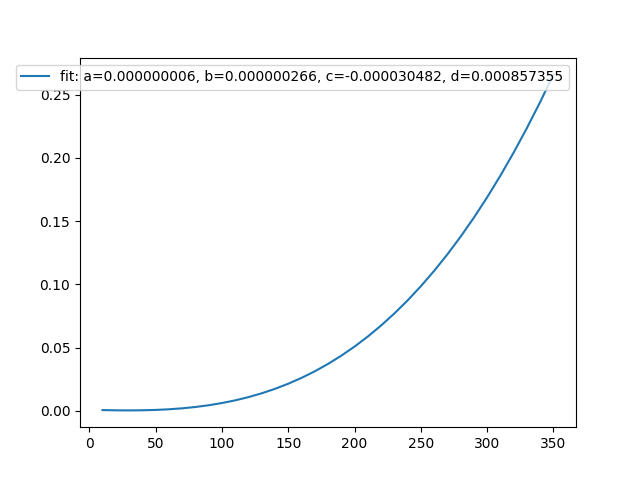
\includegraphics[width=.4\textwidth]{../graficos/floyd/floyd_elena.png}
\includegraphics[width=.4\textwidth]{../graficos/floyd/floyd_O1_elena.png}
\includegraphics[width=.4\textwidth]{../graficos/floyd/floyd_O2_elena.png}
\end{center}
\begin{center}
\includegraphics[width=.6\textwidth]{../graficos/floyd/floyd_juntas_elena.png}
\end{center}
\begin{center}
\begin{tabular}{| c | c | c | c |}
\hline
\textbf{N} & \textbf{O-} & \textbf{O1} & \textbf{O2} \\ \hline
10 & 1e-05 & 2e-06 & 2e-06 \\ \hline
20 & 6.7e-05 & 1e-05 & 9e-06 \\ \hline
30 & 0.000203 & 3.2e-05 & 2.6e-05 \\ \hline
40 & 0.000448 & 8.5e-05 & 6.4e-05 \\ \hline
50 & 0.00085 & 0.00018 & 0.000111 \\ \hline
60 & 0.001523 & 0.000245 & 0.000211 \\ \hline
70 & 0.002242 & 0.000388 & 0.000302 \\ \hline
80 & 0.003433 & 0.000628 & 0.000468 \\ \hline
90 & 0.00479 & 0.000887 & 0.000673 \\ \hline
100 & 0.006563 & 0.001241 & 0.000935 \\ \hline
110 & 0.008654 & 0.001584 & 0.001257 \\ \hline
120 & 0.011204 & 0.002048 & 0.001619 \\ \hline
130 & 0.014089 & 0.00262 & 0.00206 \\ \hline
140 & 0.017503 & 0.003243 & 0.002528 \\ \hline
150 & 0.021579 & 0.005549 & 0.003132 \\ \hline
160 & 0.025767 & 0.004884 & 0.003714 \\ \hline
170 & 0.031052 & 0.005792 & 0.004462 \\ \hline
180 & 0.036781 & 0.006995 & 0.005309 \\ \hline
190 & 0.043117 & 0.008024 & 0.006207 \\ \hline
200 & 0.050271 & 0.009325 & 0.007302 \\ \hline
210 & 0.057796 & 0.010893 & 0.00833 \\ \hline
220 & 0.066049 & 0.013512 & 0.009487 \\ \hline
230 & 0.075983 & 0.019707 & 0.010731 \\ \hline
240 & 0.08597 & 0.016271 & 0.012288 \\ \hline
250 & 0.097257 & 0.01794 & 0.013794 \\ \hline
260 & 0.11489 & 0.020119 & 0.015456 \\ \hline
270 & 0.12577 & 0.022316 & 0.017151 \\ \hline
280 & 0.135327 & 0.025045 & 0.019537 \\ \hline
290 & 0.151109 & 0.027848 & 0.022317 \\ \hline
300 & 0.173293 & 0.030866 & 0.024179 \\ \hline
310 & 0.184009 & 0.033768 & 0.026927 \\ \hline
320 & 0.209154 & 0.036916 & 0.029534 \\ \hline
330 & 0.222543 & 0.041274 & 0.032556 \\ \hline
340 & 0.243091 & 0.044321 & 0.035005 \\ \hline
350 & 0.264411 & 0.048341 & 0.037279 \\ \hline
\hline
\end{tabular}
\end{center}

\newpage
\subsection{Algoritmo floyd(Antonio)}
\begin{center}
\includegraphics[width=.4\textwidth]{../graficos/floyd/floyd_antonio.png}
\includegraphics[width=.4\textwidth]{../graficos/floyd/floyd_O1_antonio.png}
\includegraphics[width=.4\textwidth]{../graficos/floyd/floyd_O2_antonio.png}
\end{center}
\begin{center}
\includegraphics[width=.6\textwidth]{../graficos/floyd/floyd_juntas_antonio.png}
\end{center}
\begin{center}
\begin{tabular}{| c | c | c | c |}
\hline
\textbf{N} & \textbf{O-} & \textbf{O1} & \textbf{O2} \\ \hline
10 & 7e-06 & 2e-06 & 1e-06 \\ \hline
20 & 4.9e-05 & 8e-06 & 6e-06 \\ \hline
30 & 0.000138 & 2.2e-05 & 1.8e-05 \\ \hline
40 & 0.000318 & 6e-05 & 4.5e-05 \\ \hline
50 & 0.00061 & 0.000102 & 7.8e-05 \\ \hline
60 & 0.001095 & 0.000174 & 0.000135 \\ \hline
70 & 0.001595 & 0.000275 & 0.000214 \\ \hline
80 & 0.002462 & 0.000505 & 0.000333 \\ \hline
90 & 0.003471 & 0.000626 & 0.000487 \\ \hline
100 & 0.00476 & 0.000858 & 0.000677 \\ \hline
110 & 0.006267 & 0.00122 & 0.000967 \\ \hline
120 & 0.00939 & 0.0016 & 0.001387 \\ \hline
130 & 0.011997 & 0.001919 & 0.002126 \\ \hline
140 & 0.014861 & 0.002401 & 0.002966 \\ \hline
150 & 0.018396 & 0.002879 & 0.003878 \\ \hline
160 & 0.022149 & 0.003477 & 0.005903 \\ \hline
170 & 0.024497 & 0.004126 & 0.007088 \\ \hline
180 & 0.027264 & 0.00495 & 0.008384 \\ \hline
190 & 0.03225 & 0.005785 & 0.009857 \\ \hline
200 & 0.036798 & 0.006849 & 0.011657 \\ \hline
210 & 0.042716 & 0.007822 & 0.013427 \\ \hline
220 & 0.048946 & 0.009034 & 0.015228 \\ \hline
230 & 0.056021 & 0.010254 & 0.017314 \\ \hline
240 & 0.0633 & 0.011721 & 0.017356 \\ \hline
250 & 0.071353 & 0.013761 & 0.013016 \\ \hline
260 & 0.080501 & 0.015499 & 0.014667 \\ \hline
270 & 0.090349 & 0.017336 & 0.016381 \\ \hline
280 & 0.100123 & 0.019371 & 0.018226 \\ \hline
290 & 0.110743 & 0.02118 & 0.020386 \\ \hline
300 & 0.122328 & 0.023664 & 0.021195 \\ \hline
310 & 0.136484 & 0.026285 & 0.019489 \\ \hline
320 & 0.149135 & 0.02747 & 0.021226 \\ \hline
330 & 0.171821 & 0.030105 & 0.023383 \\ \hline
340 & 0.17891 & 0.033021 & 0.025405 \\ \hline
350 & 0.194148 & 0.035809 & 0.027583 \\ \hline
\hline
\end{tabular}
\end{center}


\newpage
\subsection{Algoritmo hanoi(Elena)}
\begin{center}
\includegraphics[width=.4\textwidth]{../graficos/hanoi/hanoi_elena.png}
\includegraphics[width=.4\textwidth]{../graficos/hanoi/hanoi_O1_elena.png}
\includegraphics[width=.4\textwidth]{../graficos/hanoi/hanoi_O2_elena.png}
\end{center}
\begin{center}
\includegraphics[width=.6\textwidth]{../graficos/hanoi/hanoi_juntas_elena.png}
\end{center}
\begin{center}
\begin{tabular}{| c | c | c | c |}
\hline
\textbf{N} & \textbf{O-} & \textbf{O1} & \textbf{O2} \\ \hline
1 & 2e-07 & 2.24e-07 & 1.64e-07 \\ \hline
2 & 1.67e-07 & 1.79e-07 & 1.63e-07 \\ \hline
3 & 3.33e-07 & 2.87e-07 & 2.65e-07 \\ \hline
4 & 5.75e-07 & 3.4e-07 & 3.68e-07 \\ \hline
5 & 6.74e-07 & 4.52e-07 & 4.45e-07 \\ \hline
6 & 9.91e-07 & 6.66e-07 & 5.85e-07 \\ \hline
7 & 1.647e-06 & 8.31e-07 & 8.24e-07 \\ \hline
8 & 2.758e-06 & 1.512e-06 & 1.117e-06 \\ \hline
9 & 4.436e-06 & 3.343e-06 & 1.8e-06 \\ \hline
10 & 8.186e-06 & 5.609e-06 & 3.002e-06 \\ \hline
11 & 1.5659e-05 & 8.349e-06 & 5.657e-06 \\ \hline
12 & 3.2058e-05 & 1.5869e-05 & 1.0862e-05 \\ \hline
13 & 6.0502e-05 & 3.0724e-05 & 2.0561e-05 \\ \hline
14 & 0.000119143 & 6.344e-05 & 4.19e-05 \\ \hline
15 & 0.000237536 & 0.000125609 & 8.0066e-05 \\ \hline
16 & 0.000471937 & 0.000258071 & 0.000159233 \\ \hline
17 & 0.000943677 & 0.000481852 & 0.000328443 \\ \hline
18 & 0.00184691 & 0.000994402 & 0.000635549 \\ \hline
19 & 0.00365114 & 0.00192413 & 0.00134496 \\ \hline
20 & 0.00729903 & 0.00389515 & 0.00257432 \\ \hline
21 & 0.0146018 & 0.00784956 & 0.00513506 \\ \hline
22 & 0.0292939 & 0.0155307 & 0.0101176 \\ \hline
23 & 0.0567671 & 0.0305533 & 0.0200906 \\ \hline
24 & 0.12188 & 0.0609997 & 0.0408326 \\ \hline
25 & 0.231254 & 0.122658 & 0.0810675 \\ \hline
\hline
\end{tabular}
\end{center}

\newpage
\subsection{Algoritmo hanoi(Antonio)}
\begin{center}
\includegraphics[width=.4\textwidth]{../graficos/hanoi/hanoi_antonio.png}
\includegraphics[width=.4\textwidth]{../graficos/hanoi/hanoi_O1_antonio.png}
\includegraphics[width=.4\textwidth]{../graficos/hanoi/hanoi_O2_antonio.png}
\end{center}
\begin{center}
\includegraphics[width=.6\textwidth]{../graficos/hanoi/hanoi_juntas_antonio.png}
\end{center}
\begin{center}
\begin{tabular}{| c | c | c | c |}
\hline
\textbf{N} & \textbf{O-} & \textbf{O1} & \textbf{O2} \\ \hline
1 & 1.2e-07 & 1.78e-07 & 1.36e-07 \\ \hline
2 & 1.35e-07 & 1.9e-07 & 1.57e-07 \\ \hline
3 & 2.89e-07 & 1.91e-07 & 2.03e-07 \\ \hline
4 & 3.43e-07 & 3.49e-07 & 2.94e-07 \\ \hline
5 & 5.8e-07 & 3.61e-07 & 3.9e-07 \\ \hline
6 & 7.92e-07 & 5.13e-07 & 4.65e-07 \\ \hline
7 & 1.218e-06 & 7.12e-07 & 6.87e-07 \\ \hline
8 & 1.82e-06 & 1.061e-06 & 9.75e-07 \\ \hline
9 & 3.074e-06 & 1.929e-06 & 1.429e-06 \\ \hline
10 & 6.153e-06 & 3.231e-06 & 2.336e-06 \\ \hline
11 & 1.1591e-05 & 6.328e-06 & 4.272e-06 \\ \hline
12 & 2.2193e-05 & 1.3284e-05 & 7.746e-06 \\ \hline
13 & 4.3379e-05 & 2.8738e-05 & 1.4845e-05 \\ \hline
14 & 8.624e-05 & 6.3205e-05 & 2.92e-05 \\ \hline
15 & 0.000170917 & 0.000125993 & 5.9962e-05 \\ \hline
16 & 0.00034173 & 0.000283643 & 0.000115692 \\ \hline
17 & 0.000681671 & 0.000565734 & 0.000237385 \\ \hline
18 & 0.00136209 & 0.0015293 & 0.000459186 \\ \hline
19 & 0.00285817 & 0.00373938 & 0.000997598 \\ \hline
20 & 0.00556612 & 0.00751584 & 0.00200475 \\ \hline
21 & 0.0110711 & 0.0149939 & 0.0041239 \\ \hline
22 & 0.0223174 & 0.0296655 & 0.00922785 \\ \hline
23 & 0.0420834 & 0.0304637 & 0.0183847 \\ \hline
24 & 0.0841359 & 0.0445143 & 0.0347469 \\ \hline
25 & 0.167375 & 0.0894432 & 0.057937 \\ \hline
\hline
\end{tabular}
\end{center}




\section{Algoritmos de búsqueda}
\begin{center}
\includegraphics[scale=0.6]{../graficos/ordenacion/ordenacion_antonio.png}
\end{center}

En la gráfica superior hemos representado la eficiencia empírica de todos los algoritmos de ordenación estudiados. Observando el gráfico, vemos lo eficientes que son quicksort, heapsort y mergesort con respecto a los otros.

Vemos también, que, para tamaños entre 5000 y 6000, el algoritmo de selección es más lento que el de la burbuja, pero para tamaños superiores, el algoritmo de selección es notablemente más rápido (esto se debe a que el valor del UMBRAL se encuentra entre esos valores). Además observamos que el algoritmo de inserción siempre es más rápido que el de selección y el de la burbuja.

\begin{center}
\includegraphics[scale=0.5]{../graficos/ordenacion/ordenacion_sort_only_antonio.png}
\end{center}

Debido a que en la anterior imagen no podemos comparar adecuadamente los algoritmos quicksort, mergesort y heapsort, hemos generado otra gráfica con ellos solos. 

Observamos ahora que para tamaños menores a 2000 el algoritmo mergesort es más lento que los demás, pero a partir de ese tamaño se hace evidente que es el mejor algoritmo de ordenación de todos los vistos aquí.

\section{Variación del ajuste según la función}

\begin{center}
\includegraphics[scale=0.7]{../graficos/ordenacion/ajuste_antonio.png}
\end{center}

En la gráfica de arriba hemos realizado el ajuste correspondiente al algoritmo de la burbuja optimizado con la opción $O2$, pero esta vez ajustándolo a otras funciones. Como vemos, la calidad del ajuste es pésima, la función $f(x)=x^3$ sale tan alejada de los datos que ni siquiera se muestra en el gráfico, y la función logarítimica no se acerca mucho tampoco. Sin embargo la función $x^2$ se ciñe perfectamente a los datos tomados. Aquí se ve la importancia de realizar un buen estudio teórico de la eficiencia antes de realizar el estudio empírico.


\section{Variación de la eficiencia según el ordenador donde se ejecuta}

A continuación vemos unas gráficas donde podemos ver que la eficiencia teórica de los algoritmos se mantiene sin importar el ordenador en el que sea ejecutado. Lo único que varía son los coeficientes, que serán mejores según las prestaciones del ordenador, en este caso podemos ver que el ordenador de Antonio ejecuta mejor la mayoría de los algoritmos al tener unas mejores prestaciones que el de Elena, aunque esto no pasa en todos los casos.

\begin{figure}
\centering
\includegraphics[scale=0.7]{../graficos/distintos/burbuja.png}
\caption{Burbuja}
\end{figure}

\begin{figure}
\centering
\includegraphics[scale=0.7]{../graficos/distintos/insercion.png}
\caption{Inserción}
\end{figure}

\begin{figure}
\centering
\includegraphics[scale=0.7]{../graficos/distintos/seleccion.png}
\caption{Selección}
\end{figure}

\begin{figure}
\centering
\includegraphics[scale=0.7]{../graficos/distintos/quicksort.png}
\caption{Quicksort}
\end{figure}

\begin{figure}
\centering
\includegraphics[scale=0.7]{../graficos/distintos/heapsort.png}
\caption{Heapsort}
\end{figure}

\begin{figure}
\centering
\includegraphics[scale=0.7]{../graficos/distintos/mergesort.png}
\caption{Mergesort}
\end{figure}

\begin{figure}
\centering
\includegraphics[scale=0.7]{../graficos/distintos/floyd.png}
\caption{Floyd}
\end{figure}

\begin{figure}
\centering
\includegraphics[scale=0.7]{../graficos/distintos/Hanoi.png}
\caption{Hanoi}
\end{figure}


\end{document}